\RequirePackage[l2tabu,orthodox]{nag}

% TODO: decide if one-sided/two-sided
%\documentclass[headsepline,footsepline,footinclude=false,fontsize=11pt,paper=a4,listof=totoc,bibliography=totoc,BCOR=12mm,DIV=12]{scrbook} % two-sided
\documentclass[headsepline,footsepline,footinclude=false,oneside,fontsize=11pt,paper=a4,listof=totoc,bibliography=totoc]{scrbook} % one-sided

\usepackage{amsmath}
\usepackage{algorithm, setspace}
\usepackage[noend]{algpseudocode}
\usepackage{xcolor}
\usepackage{pgf-pie}

\usepackage{mathtools}


% TODO: change citation style in settings
\input{settings}

\usepackage{cleveref}

% TODO: change thesis information
\newcommand*{\getUniversity}{Technische Universität München}
\newcommand*{\getFaculty}{School of Computation, Information and Technology Informatics}
\newcommand*{\getTitle}{Speeding-up Post-Quantum Cryptography on an RSA Co-Processor}
\newcommand*{\getTitleGer}{Beschleunigung der Post-Quantum-Kryptographie auf einem RSA-Coprozessor}
\newcommand*{\getAuthor}{Horia Ionut Turcuman}
\newcommand*{\getDoctype}{Master's Thesis in Informatics}
\newcommand*{\getSupervisor}{Prof. Dr. Claudia Eckert}
\newcommand*{\getAdvisor}{Felix Fritz Oberhansl, Tobias Stelzer}
\newcommand*{\getSubmissionDate}{19.09.2023}
\newcommand*{\getSubmissionLocation}{Munich}

\newcommand\todo[1]{\textcolor{red}{TODO: #1}}

\newcommand{\Z}{\mathbb{Z}}
\newcommand{\Zq}{\mathbb{Z}_q}
\newcommand{\R}{\mathbb{Z}[X]/(X^n + 1)}
\newcommand{\Rq}{\mathbb{Z}_q[X]}
\newcommand{\Rnq}{\mathbb{Z}_q[X]/(X^n + 1)}
\newcommand{\Ryq}{\mathbb{Z}_q[Y]/(Y^{n/t} + 1)}
\newcommand{\Ryxq}{\mathbb{Z}_q[Y]/(Y^{n/t} + 1)[X]/(Y-X^t)}

\newtheorem{theorem}{Theorem}[section]
\newtheorem{definition}{Definition}[section]

\begin{document}

% Set page numbering to avoid "destination with the same identifier has been already used" warning for cover page.
% (see https://en.wikibooks.org/wiki/LaTeX/Hyperlinks#Problems_with_Links_and_Pages).
\pagenumbering{alph}
\input{pages/cover}

\frontmatter{}

\input{pages/title}
\input{pages/disclaimer}
\addcontentsline{toc}{chapter}{Acknowledgments}
\thispagestyle{empty}

\vspace*{20mm}

\begin{center}
{\usekomafont{section} Acknowledgments}
\end{center}

\vspace{10mm}

%TODO: Acknowledgments

I would like to thank my supervisors Felix Fritz Oberhansl and Tobias Stelzer who guided me through the process of writing this thesis and helped me with explanations, ideas and resources. I also want to thank my parents who have long supported me and continue to do so.

\cleardoublepage{}

\chapter{\abstractname}

%TODO: Change order: first background then my work then results

Public-key cryptography has been widely employed for securing the digital world and enabling critical applications. In constrained devices, dedicated co-processors provide functionality required by popular schemes such as RSA and ECC. These schemes became obsolete with the advent of the famous Shor's algorithm that leverages the power of quantum computers to break their fundamental assumptions. Quantum-resistent schemes come as an answer to the threat of quantum computers to security by providing new cryptographic constructs that do not rely on assumptions that the Shor's algorithm can invalidate. The large scale adoption of post-quantum cryptographic schemes that were nominated to become the new standard is hindered by the fact that a large number of them require different functionality than the old dedicated cryptographic processors offer. Since these devices will still be in-use for many years to come, it is important to secure them for the future by repurposing deployed cryptographic co-processors.
 
In this thesis we implement the Kronecker+ polynomial multiplication algorithm tuned for the CRIYSTALS-Dilithium post-quantum, RLWE-based signature scheme, on the OpenTitan Big Number Accelerator (OTBN). The Kroneker+ algorithm presented by Bos et al. at USENIX 2022 builds on top of the functionality offered by common cryptographic co-processors and enables efficient polynomial multiplication which is what many new RLWE-based schemes such as Dilithium require. We benchmark the implementation for various parameter and compare the results with other implementations of the chosen scheme.
\microtypesetup{protrusion=false}
\tableofcontents{}
\microtypesetup{protrusion=true}

\mainmatter{}

% !TeX root = ../main.tex
% Add the above to each chapter to make compiling the PDF easier in some editors.

\chapter{Introduction}\label{chapter:introduction}

\section{Motivation}

Embedded devices have become indispensable for many people and organizations, ever more use cases being explored and solutions being deployed. Their role is increasingly more important in the day to day life, fabrics and many other environments, sometimes being key solutions and other times enabling unprecedented possibilities. Their wide application makes their security a critical point which has been continuously improved in the past. Notably, public-key cryptography is an essential cryptographic method that secures the communication inter-devices, with servers or clouds and with terminals. Public-key cryptography is commonly used in protocols that initiated communication by establishing secure channels in insecure environments. The expensive computations required by established public-key schemes such as Rivest–Shamir–Adleman (RSA)~\parencite{10.1145/359340.359342} and Elliptic Curve Cryptography (ECC)~\parencite{10.1007/3-540-39799-X_31} are, in many IoT and embedded devices, deferred to dedicated hardware accelerators that can handle large integer arithmetic efficiently. This is achieved by instruction sets and hardware-design aimed for large number computations. Beside the algorithmic efficiency of the cryptographic schemes, these processors' ability to provide efficient large computations is another key factor in securing communication. Application domains requiring real-time communication critically depend on such considerations, and speed is important in many other areas as well. It is then no wonder that much work has been put into building and optimizing such processors, cryptographic schemes and their implementations. Nowadays many of the challenges related to providing fast secure communication have been tackled and good solutions exist. In the future on the other hand, quantum computers threaten to break the established security for which so much work has been dedicated.

Cryptographic schemes such as RSA and ECC are based on various unproven assumptions from which their entire security comes from. Even if the assumptions could not be proven, these schemes have been widely accepted and deployed counting on the fact that nobody was able to break them for a long time. This changed with the emergence of Shor's algorithm~\parencite{365700} which breaks the assumptions used in the two most popular schemes. Quantum computers are momentarily not able to work with large numbers, hence our security is still in place. It is also not clear how much time it would take to construct powerful enough machines but what is sure is that if and when that happens, the world needs to be ready for it. For this reason, quantum-resistant schemes have been and are developed, tested and improved in order to come up with standards for the 'new' security. With this goal, the US National Institute of Standards and Technology (NIST), in their effort to speed up the unavoidable transition, called for and assessed new quantum-resistant schemes. They selected the key encapsulation mechanism  CRYSTALS-Kyber~\parencite{cryptoeprint:2017/634} and the digital signature schemes CRYSTALS-Dilithium~\parencite{cryptoeprint:2017/633}, FALCON~\parencite{Soni2021} and SPHINCS+~\parencite{10.1007/978-3-662-46800-5_15} as the winners. The previous cryptographic schemes used in so many applications and devices are now expected to be exchanged for one of the winning schemes. This migration is expected to take many years, though eventually, anyone that wants to stay secure will replace the old cryptography.

As important as this transition now is, it is also very challenging to adopt the new schemes. From the seven finalists, none of them require the large number arithmetic as the previous schemes did and what the in-circulation co-processors are built for. New dedicated hardware is and will continue to be developed but immediately replacing all old processors in our devices is too costly and unrealistic, therefore, the challenge of repurposing these pieces of hardware emerges. Many of the new schemes have in common the fact that they are based on ring-based lattice cryptography which requires fast multiplication of polynomials with integer coefficients. This kind of cryptography proved to lead to state-of-the-art schemes, hence researchers worked on ways of mapping polynomials to large integers and back in order to take advantage of the existent hardware capabilities. Indeed, efficient algorithms for this tasks exist and have been successfully applied to some of the secure schemes on various platforms and hardware accelerators. 

\section{Previous work}

One simple algorithm that maps polynomials from $\Z[X]$ to large integers and the other way around is Kroneker substitution~\parencite{10.1007/3-540-11607-9_1}. It claims that evaluating two polynomials at a large enough integer point and multiplying the evaluation values yields a number that corresponds to exactly one polynomial given the point of evaluation $x$. Moreover, clever modulo $x$ operations allow for recovering this polynomial. This already allows implementing the new schemes using the old co-processors but is not very efficient due to the too large resulting integer which drastically decrease the multiplication performance, as contemporary co-processors are built for integer sizes of RSA/ECC, these being considerably smaller.

Harvey's ~\parencite{HARVEY20091502} improvements to Kroneker substitution work with polynomials from the polynomial ring $\R$ and allow for decreasing the resulting integers sizes by a factor of 2 or 4 at the expense of having to perform more multiplications (by a factor of 2 respectively 4). They work by evaluating the polynomials at the roots of unity in $\Z$, namely 1 and -1. These optimizations become more advantageous the larger the integers are.~\parencite{cryptoeprint:2018/425} gives a description of using these methods for the purpose of implementing RLWE-based schemes using RSA-dedicated co-processors, and it is important to note that they re already practical, an actual implementation for a specific scheme on a specific processor being presented in~\parencite{10.1007/978-3-030-57808-4_21}.

Besides Harvey's method, there exist a couple more ways of improving Kroneker substitution by combining it with various ways of looking at the initial polynomial. Among others, the methods of Karatsuba~\parencite{karatsuba}, Toom-Cook~\parencite{Cook1969ONTM}, Schönhage-Strassen~\parencite{strassen} and Nussbaumer~\parencite{Nussbaumer1980FastPT} are the most prominent. A survey of such methods is given by Bernstein~\parencite{10.1007/978-3-030-57808-4_21}.

Recent research yielded a new approach that beats many of the old ones from multiple points of view: from number of multiplications and integer sizes to actual running speed. Kroneker+~\parencite{cryptoeprint:2020/1303} generalizes the Harvey's algorithm for polynomials in $\Rnq$ where, after Kroneker substitution which yields values in $\Zq$, more roots of unity are available.  Significant advantages show up for larger integers when comparing to Harvey's method. Kronecker+ decreases the size of integers to be multiplied and trades multiplications for more efficient additions and bit shifts by exploiting the underlying ring structure. To have a rough idea, given a trade-off parameter $t$, when the cost of $b$-bit integer multiplication is $M(b)$, the cost of the algorithm is $t \cdot M(b / t) + \mathcal{O}(t)$. Assuming that $M(b)$ is significantly smaller for smaller $b$, it makes sense to use a larger $t$ as long as the overhead factor $\mathcal{O}(t)$, which scales approximately with $t \cdot log(t)$, stays small. The ring $\Rnq$, on which Kroneker+ operates, allows for clever simplifications and efficient implementations. It's effectiveness and the fact that many important post-quantum cryptographic constructions work with polynomials in this ring, makes Kroneker+ the algorithm of choice for our goal of using the old-fashioned OTBN co-processors with the new schemes.~\autoref{tab:comparison1} from~\parencite{cryptoeprint:2020/1303} shows a comparison between different methods.

%This effectively means that that one can to work with resulting numbers of sizes smaller by any factor $t = 2^\tau$ compared to plainly applying Kroneker substitution, at the expense of having to multiply $t$ such numbers.%


\begin{table}[htpb]
  \caption[]{Table 1 from~\parencite{cryptoeprint:2020/1303}. Comparison between various polynomial multiplication methods via large integer multiplication. The parameter n is the polynomial degree, $2^l$ is the point of evaluation for Kroneker substitution, t is a parameter of the algorithms, controlling the trade-off between integer size and number of multiplications.}\label{tab:comparison1}
  \centering
  \begin{tabular}{l l l l}
    \toprule
      Algorithm & \# Muls & \# Bits\\
    \midrule
      Kroneker (KS1) & 1 & $ln + 1$ \\
      Harvey (KS2/KS3) & 2 & $ln / 2 + 1$ \\
      Harvey (KS4) & 4 & $ln / 4 + 1$ \\
      Kroneker + Karatsuba & $3^{log(t)}$ & $(ln + 1) / t$ \\
      Kroneker + Toom-Cook-t & $2t - 1$ & $ (ln + 1) / t$ \\
      Kroneker + Schön.-Strassen & $t$ & $ln / t + t + 1$ \\
      Nussbaumer + Kroneker & $2t$ & $ln/t + 1$ \\
      Kroneker+ & $t$ & $ln/t + 1$ \\
    \bottomrule
  \end{tabular}
\end{table}

\break


\section{Contribution}

The goal of this work is to inspire further implementations for other schemes and provide a basis for production-ready version so that eventually the scheme will be used by embedded devices. The Kroneker+ algorithm is implemented and fine tuned for the Dilithium digital signature scheme, on the OpenTitan Big Number Accelerator (OTBN). The winners of the NIST competition being announced, it is important to fine tune the state-of-the-art algorithms for them in order to move one step closer to wide adoption of the new schemes. The Kroneker+ can be efficiently implemented only once the parameter set is fixed, hence, by considering various aspects of the scheme, the multiplication algorithm and implementation optimizations enabled by different parameters, two sets of parameters that allows for a highly efficient implementation are chosen. Since one of the principal time consumers of the Kroneker+ method is the Number Theoretic Transform (NTT) computation, this work focuses on combining and adapting a few implementations of this transformation in order to achieve the most suitable version from both an implementation perspective as well as a running time perspective. Furthermore, a working and optimized implementation using the instruction set provided by the OTBN processor is developed and the reader is guided step by step through it. Challenges such as using a multiplier and other instructions that work on smaller bit lengths than the required integer sizes of the algorithm, manually implementing modulo reduction in an efficient way and determining the minimal required spots where it has to be applied, reducing the amount of data memory accesses by combining steps and finding workarounds when specific functionalities as register indexing are mixing show up and are addressed in this thesis. In the end an analysis including benchmarks of various steps, comparisons with other polynomial multiplication algorithms and comparisons of two different sets of parameters are is provided in order to aid in identifying further improvements of the code.

\chapter{Background}\label{chapter:background}

Throughout this section we will deal with polynomials from the ring $\Rnq$ since this is the setting in which the Dilithium scheme operates. Many of the discussed considerations do apply to the more general settings of $\R$, $\Z[X]$ or even replacing $\Z$ by a general ring under the assumption that the necessary inverses exist. We start by introducing the reader to arguably simpler technique of mapping polynomials to integers and back, and continue with various ways of viewing the polynomials such that this conversion and the multiplication in the integers domain become most efficient. We include with each method high-level pseudocode but we keep the implementation details and OTBN instruction set specific approaches for the implementation chapter.

\section{Notation}

In this thesis a few notations and signs are used to simplify the descriptions and add more details. $M(b)$ denotes the multiplication time for multiplying two b-bit numbers and it is assumed to be an increasing function. The number $t$ is the degree of the polynomial on which the NTT is computed and acts as a tradeoff parameter between the integer size, NTT computation cost and the multiplication cost. The input polynomial degree will be denoted by $n$ and $q$ will be the modulus by which coefficients of the output polynomial need to be reduced. The unique integer $\hat{a}$ = a $mod$ b such that $0 \leq \hat{a} < b$ is denoted by a $mod^+$ b. A polynomial $f \in \Rnq$ will be written in it's usual form $f = \sum_{i=0}^{n-1} f_i X^i$ as well as in coefficient-vector form $f = (f_0, \ldots, f_{n-1})$. We denote the coefficient-wise multiplication of 2 polynomials or sequences by $\cdot$ and the convolution operation by $*$.

The space of vectors of polynomials on which Dilithium works is denoted by $S_{q, \alpha}^k = \{w \in \Rnq$ s.t. $0 \leq w_i < \alpha\}^k$ be the space of vectors of polynomials limited by $\alpha$.

\section{Dilithium Digital Signature Scheme}

Dilithium~\parencite{cryptoeprint:2017/633} is a lattice-based cryptographic scheme that works with polynomials from $\Rnq$ for $q = 8380417 = 2^{23} - 2^{13} + 1$ and $n = 256$. Many other important schemes are operating on lattices in their inner workings, therefore performance improvements to the lattice specific operations can transfer to other schemes and have a significant impact. The bottleneck in this type of cryptographic schemes is the matrix-vector multiplication of a matrix $A \in (\Rnq)^{m \times k}$ and a vector $v \in S_{q, \alpha}^k$ with $\alpha = (q - 1) / 16$.~\autoref{tab:parameters1} from \parencite*{cryptoeprint:2017/633} contains the values of these parameters for different security levels. Since $m$ and $k$ are small, the actual factor that makes the matrix vector multiplication expensive is not the number of operations, rather the actual polynomial multiplication. Different techniques exist for speeding this computation up, one of them being the $NTT$ which is used in Dilithium and which maps polynomials to another domain ($NTT$ domain) where polynomial multiplication becomes pairwise coefficient multiplication. For performance reasons, the scheme generates the numbers used for the coefficients of the polynomials directly in the $NTT$ domain. To apply another method for speeding up the multiplication, one would have to tweak the scheme to generate the numbers in the usual domain.

It is important to note that the modulo polynomial $X^n + 1$ was chosen such that mathematical formulas and the implementation simplify and can be optimized. The fact that $X^n = -1\ \bmod (X^n + 1)$ makes the implementation of the modulo operation trivial by replacing $X^n$ with $-1$. The fact that there is a plus instead of a minus is also important for the implementation of the $NTT$, allowing for clever optimizations.


\begin{table}[htpb]
    \caption[]{Dilithium parameters taken from \parencite*{cryptoeprint:2017/633} }\label{tab:parameters1}
    \centering
    \begin{tabular}{l l l l l l}
      \toprule
        Security level & n & q & m & k & $\alpha$\\
      \midrule
        weak & 256 & 8380417 & 3 & 2 & 523776 \\
        medium & 256 & 8380417 & 4 & 3 & 523776 \\
        recommended & 256 & 8380417 & 5 & 4 & 523776 \\
        very high & 256 & 8380417 & 6 & 5 & 523776 \\
      \bottomrule
    \end{tabular}
  \end{table}

\section{Kroneker substitution}

Kroneker substitution \parencite*{KroneckerGrundzgeEA} is a classical technique for reducing polynomial arithmetic to integer arithmetic. The approach is based on the observation that evaluating a polynomial at an integer point allows for recovering the polynomial by successive modulo operations and divisions by this value. If a \emph{large enough} evaluation point is used, the coefficients are packed in such a way that each one has a large \emph{room}. When multiplying two polynomials packed in such a way, the \emph{large room property} eliminates the possibility of having carries from one \emph{room} to the next effectively not allowing coefficient to mix with one another. Take for example $f(X) = 3 X + 2 \implies f(100) = 302$ and $g(X) = 5 X + 10 \implies g(100) = 510$. Then $f(100) \cdot g(100) = 302 \cdot 510 = 154020$ and $f(X) \cdot g(X) = 15 X^2 + 40 X + 20$ which can be recovered from 154020 by grouping the digits. This process becomes less straight forward when the polynomials contain negative coefficients but it turns out that it is also possible to work with them. Grouping the digits can be changed with applying modulo operations and divisions by the evaluation point when the value is not as nice as in the previous example. For performance reasons, this point is usually chosen to be $2^l$ for some $l \in \Z$ large enough. 

Kroneker substitution can be used for both multiplications and additions, and also for computations modulo $X^n + 1$ as stated in~\parencite{cryptoeprint:2020/1303}. Given a certain sequence of operations (e.x. $a \cdot b + c \cdot d + e$ with $a, b, c, d, e \in \Rnq$), an evaluation point that makes the method work correctly for a certain set of polynomials depends only on an upper and lower bound on the coefficients of the resulting polynomial. These can be computed from upper and lower bounds on the coefficients of the polynomials in the given set.~\parencite{cryptoeprint:2018/425} details a couple of results on choosing evaluation points in various settings.~\parencite{cryptoeprint:2020/1303} points out that, although the coefficients of the polynomials $f \cdot g$ and $f \cdot g$ mod $X^n + 1$ are different, since any coefficient of the $f \cdot g$  is the sum of at most $n$ products of coefficient from $f$ and $g$ while coefficients in the $f \cdot g$ mod $X^n + 1$ are sums of exactly $n$ such coefficient products, the minimal evaluation point for Kroneker substitution is the same for usual multiplication and multiplication modulo $X^n + 1$. In other words, the value of $l$ when the computations are performed modulo $X^n + 1$ can be chosen to be the same as if no modulo reduction was performed. Bellow, algorithm \cref{alg:snort} and algorithm \cref{alg:sneeze} taken from ~\parencite*{cryptoeprint:2018/425} describe the $SNORT$ and $SNEEZE$ operations respectively.


\begin{algorithm}
    \caption{SNORT operation of Kroneker substitution}
    \label{alg:snort}
    \begin{algorithmic}[1]
    
    \Procedure{SNORT}{$g, f \in \Z[X]$, bitlength $l$}

        \Return $g(2^l)$ $mod^{+}$ $f(2^l)$
    
    \EndProcedure
    
    \end{algorithmic}
\end{algorithm}

\begin{algorithm}
    \caption{SNEEZE operation of Kroneker substitution}
    \label{alg:sneeze}
    \begin{algorithmic}[1]
    
    \Procedure{SNEEZE}{$m \in \Z[X]$ monic, $G \in \{0, \dots, f(2^l) - 1\}$, bitlength $l$}

        $n \leftarrow$ deg(f)

        $G[-1] = G$

        \For{$i = 0, \dots, n - 1$}

            \State $e[i] \leftarrow G[i - 1]$ $mod^+$ $2^l$ 
            \State $G[i] \leftarrow (G[i - 1] - e[i]) / 2^l$ 
            \If{$e[i] > 2^{l - 1}$} \Comment{negative coefficients}
                \State $e[i] \leftarrow e[i] - 2^l$
                \State $G[i] \leftarrow G[i] + 1$
            \EndIf
        \EndFor

        \For{$i = 0, \dots, n - 1$}
            \State $e[i] \leftarrow e[i] - f_i \cdot G[n - 1]$
        \EndFor

        \Return $e[0, \cdots n - 1]$
    
    \EndProcedure
    
    \end{algorithmic}
\end{algorithm}
 
\section{Fourier Transformation}

To set up the stage for the upcoming descriptions, let $f = \sum_{i=0}^{n - 1} X^i$, $g = \sum_{i=0}^{n - 1} X^i$ be in $\Rnq$. The purpose of all the discussed procedures is to compute the multiplication $h = f * g $ $mod$ $(X^n + 1)$. The heavy operation is the polynomial multiplication, the modulo reduction being much faster. Therefore, multiplication in $\Rnq$ would not be significantly slower than multiplication in $\Rq$ but the modulo reduction by  $X^n + 1$ proves to be important for the mathematical details of the described methods and allows for faster multiplication algorithms.

\subsection{Discrete Fourier Transform}

The discrete Fourier transform (DFT) is an incredibly widely used tool with applications in many domains, most notably being signal processing and computing convolutions. It transforms a complex-valued, continuous function from it's original domain (called time domain in physical applications) to another domain (called frequency domain in the same application) where different properties hold. For the purpose of polynomial multiplication, the convolution theorem~\parencite{enwiki:1171895737} is the most important property that allows for important speed up. The theorem says that a convolution of two functions in their domain of definition can be computed by computing the inverse of the point-wise multiplication of the two transformed functions. The following equation summarizes this description:

\begin{equation*}
    f * g = DFT^{-1}(DFT(f) \cdot DFT(g))
\end{equation*}

The discrete-time Fourier transform (DTFT) is a modified DFT that is applicable to discrete finite sequences of complex numbers. The convolution theorem holds for this transform as well and since polynomial multiplication is in fact a convolution operation of the sequences represented by the polynomial coefficients. Because of this, the DTFT can be employed to speed up this multiplication. The time complexity of plain polynomial multiplication is $\mathcal{O}(n^2)$ where n is the polynomial degree, and that of the multiplication via DTFT is $\mathcal{O}(n \log(n))$ so it is a significant theoretical improvement. Since efficient implementations of the DTFT are also possible, the DTFT became also a widely used tool in practice. A very good description of the $DTFT$ from an algorithmic point of view can be found in the Introduction to Algorithms book~\parencite{10.5555/1614191} in the chapter about Fast Fourier Transformation. That introduction leads to the intuitive, recursive implementation of the algorithm. Since the $DTFT$ is used in uncountable many time-critical applications, several mathematical and algorithmic optimizations have been developed in the past.

\subsection{Cyclic Convolution-based Number Theoretic Transform}

The $NTT$ method is a central component of this work. The method is a particular case of the famous DTFT which is applied in a finite field as proposed by Pollard~\parencite{Pollard1971TheFF}. A survey that presents the $NTT$ and a few of it's variants in a mathematical way is~\parencite{liang2022number}. It is not possible to implement all optimizations at once because some are mutually exclusive, hence there exist a couple of ways to implement the $NTT$, some being more cache-aware, others focusing on reducing the number of computations and so on. This section provides a short introduction to the $NTT$ and lists possible optimizations. The section starts by explaining a simple algorithm and it's recursive implementation and continues with the equivalent iterative implementation and lastly a very efficient variant is described.

The first important thing to understand is what can the NTT do. Besides other things, in the context of polynomial multiplication it is a method to efficiently compute convolutions. This section identifies two types of convolutions and the next section will explain a third one. The first one is the linear convolution:

\begin{definition}[Linear Convolution]
    The linear convolution of two polynomials $f, g \in \Rq$ of degree n is their usual multiplication $h = f * g = \sum_{k=0}^{n-1} h_k X^k$ where $h_k = \sum_{i=0}^k f_i \cdot g_{k-i} \mod q$. To compute the product in $\Rq / (m(X))$ for some polynomial $m(X)$, one can compute the linear convolution $h = f * g \in \Rq$ and then compute $h$ mod $m(X)$. 
\end{definition}

The naive way of computing the coefficients $h_k$ of a linear convolution is to directly evaluate the sum for each of them. The number theoretic transformation with $2n$ evaluation point, i.e. $NTT_{2n}$, is an alternative to this direct computation that is more efficient while producing the same result. The second type of convolution is the cyclic convolution:

\begin{definition}[Cyclic Convolution]
    The cyclic convolution of two polynomials $f, g \in \Rq/(X^n - 1)$ is their usual multiplication in the underlying ring: $h = f * g = \sum_{k=0}^{n-1} h_k X^k$ where $h_k = \sum_{i=0}^k f_i \cdot g_{k-i} + \sum{i=k + 1}^{n-1} f_i + g_{k+n-i} \mod q$. 
\end{definition}

Similar with the linear convolution, the cyclic convolution can be computed efficiently using a number theoretic transformation with n evaluation points, i.e. $NTT_n$. This transformation is defined below:

\begin{definition}[NTT and Inverse NTT]
    Fixing a number $n$, and given a polynomial $f = \sum_{i=0}^{n-1} f_i X^i \in \Rq$ of degree bound $n$, it's transformed version is:
    
    \begin{equation*}
        F = NTT_n(f) = \sum_{k=0}^{n-1} F_k X^k
    \end{equation*}
    
    where $F_k = f(\omega_n^k) = \sum_{i=0}^{n-1} f_i \cdot w_n^{ki}$ and $w_n$ is the n-th principal unity root in $\Zq$. These roots exist if $n = 1\ mod\ q$. The inverse $NTT$ of a polynomial $F \in \Rq$ of degree bound $n$ is:
    
    \begin{equation*}
        f = INTT_n(F) = n^{-1} \sum_{i=0}^{n-1} f_i X^i
    \end{equation*}

    where $f_i = F(\omega_n^{-i}) = \sum_{k=0}^{n-1} F_k \cdot w_n^{-ik}$.
\end{definition}

\begin{theorem}
    It holds that $f = INTT_n(NTT_n(f))$.
\end{theorem}

Given the definition of the NTT, it is educative to look back at the linear convolution. The usual product of two polynomials of degree $n$ is a polynomial of degree $2n$. In order to obtain such a polynomial, the NTT with $2n$ evaluation points needs to be used. In order to use such an NTT, the input polynomials need to have $2n$ degree which can be achieved by padding them with n 0s. To compute the cyclic convolution, the NTT with only n evaluation points is needed, hence no padding is required.

Directly evaluating all sums in the above definition leads to $\mathcal{O}(n^2)$ computations which can be more efficiently computed through the so called fast fourier transformation ($FFT$) algorithm. Variants of it are presented in the subsequent sections. For the moment, in order to develop an understanding of the NTT, the next section presents an alternative way of representing a polynomial and points out how the transformation between the usual representation and the new one can be achieved through the NTT.

\subsubsection{Point value representation}

The naive way of computing the coefficients $h_k$ of a linear convolution is to directly evaluate the sum for each of them. This takes $\mathcal{O}(n^2)$ time and needs to be improved. A more clever solution is to represent the polynomials in a different way as presented in~\parencite{10.5555/1614191}:

\begin{definition}[Point-Value Representation]
    The point-value representation of a polynomial $f = \sum_{i=0}^{n-1} f_i X^i \in \Rq$ (or $\mathbb{Z}[X]$ or $\Rnq$) is any sequence $\boldsymbol{f}$ = ($(x_0, f(x_0))$, $(x_1, f(x_1))$, $\ldots$, $(x_{n-1}, f(x_{-1}))$) where the evaluation points $x_k$ are distinct.
\end{definition}

The process of finding a sequence $(x_0, \ldots, x_{n-1})$ of evaluation points and evaluating the polynomial at these points is called evaluation. The inverse process, i.e. finding a polynomial $f$ of degree at most $n$, from a sequence $((x_0, y_0), \ldots, (x_{n-1}, y_{n-1}))$ such that $f(x_k) = y_k$ is called interpolation and can be algorithmically implemented. The uniqueness of such a polynomial is guaranteed by theorem 30.1 from~\parencite{10.5555/1614191}. Both evaluation and interpolation can be naively implemented in $\mathcal{O}(n^2)$ but, as we will see, this can be sped up to $\mathcal{O}(n \log(n))$.

The point-value representation is often used for fast polynomial multiplication since $h(x_k) = f(x_k) \cdot g(x_k)$, therefore to compute the point-value representation of the product polynomial $h$, pairwise multiply the elements of the point-value representation of $f$ and $g$. The only issue with this is that when the terms $f$ and $g$ have at most degree $n$, their product will be of degree at most $2n$, therefore possibly larger than $n$. Hence, to obtain a representation of $h$ one needs to use $2n$ evaluation points even if that is redundant for $f$ and $g$ separately. The multiplication can be then carried out by first evaluating $f$ and $g$ at $2n$ points, pairwise multiplying the values and interpolating the resulting point-value representation. The following visualization can be helpful:

\begin{equation*}
    \begin{rcases}
        \begin{aligned}
        f &\mapsto ((x_0, y_0), \ldots, (x_{2n}, y_{2n})) \\
        g &\mapsto ((x_0, y^{'}_0), \ldots, (x_{2n}, y^{'}_{2n}))
        \end{aligned}
    \end{rcases} \mapsto ((x_0, y_0 \cdot y^{'}_0), \ldots, (x_{2n}, y_{2n} \cdot y^{'}_{2n})) \mapsto f \cdot g 
\end{equation*}

As already pointed out, a point-value representation exists for any sequence of distinct evaluation points. To speed up the evaluation and interpolation, one can work with the $2n$ unity roots $\omega_{2n}^0,\ \omega_{2n}^1,\ \ldots,\ \omega_{2n}^{2n}$ where $\omega_{2n}$ is the principal $2n$ unity root. For these points, the evaluation is exactly the $NTT$, and we have:

\begin{equation*}
    INTT_{2n}(NTT_{2n}(f)) = f = interpolation_{2n}(eval_{2n}(f)) = interpolation_{2n}(NTT_{2n}(f)) 
\end{equation*}

Since this holds for all $f$, the interpolation and $INTT$ are also the same. Computing the $NTT$ and $INTT$ can be done through the Cooley-Tukey Butterfly algorithm of complexity $\mathcal{O}(n \log n)$ as presented in the next section.

\subsubsection{Recursive Cooley-Tukey Butterfly}

There are many variants of the fast fourier transformation algorithm, this section presenting a simple, recursive variant inspired from~\parencite{10.5555/1614191}. The method works in asymptotic time $\mathcal{O}(n \log(n))$. While other variants can deal with arbitrary values of $n$, this version and all upcoming ones are only working with $n$ being a power of 2, which is enough for our purposes.

The recursion takes as input a degree $n-1$ polynomial $f = \sum_{i=0}^{n-1} f_i \cdot X^i$ and constructs two new polynomials as follows:

\begin{align*}
    f_{even} &= f_0 X^0 + f_2 X^1 + f_4 X^2 + \ldots + f_{n-2} X^{n/2-1} \\
    f_{odd} &= f_1 X^0 + f_3 X^1 + f_5 X^2 + \ldots + f_{n-1} X^{n/2-1} 
\end{align*}

It is easy to see that $f(x) = f_{even}(x^2) + x f_{odd}(x^2)$. To evaluate $f$ at the unity roots $w_n^0, w_n^1, \ldots$, $w_n^{n-1}$, one needs to evaluate the two new polynomials at $(w_n^0)^2, (w_n^1)^2$, $\ldots\ (w_n^{n-1})^2$ and combine the results as shown. This list contains only $n/2$ distinct values since $w_n^i = w_n^{n+i}$. Further, the equality $w_n^{2i} = w_{n/2}^i$ holds, hence the procedure evaluates the new polynomials at the $n/2$ $n/2$-roots of unity. Even more, note that $w_n^{n/2 + i} = w_n^{n/2} \cdot w_n^i = - w_n^i$ since $w_n^{n/2} = -1$. The following shows how the recursion works for $0 \leq i < n/2$:

\begin{equation*}
    f(\omega_n^i) = f_{even}(\omega_n^{2i}) + \omega_n^i \cdot f_{odd}(\omega_n^{2i}) = f_{even}(\omega_{n/2}^{i}) + \omega_n^i \cdot f_{odd}(\omega_{n/2}^{i}) 
\end{equation*}

For $n/2 \leq i < n$ we get:

\begin{align*}
    f(\omega_n^i) &= f_{even}(\omega_n^{2i}) + \omega_n^i \cdot f_{odd}(\omega_n^{2i}) \\ 
    &= f_{even}(\omega_{n/2}^{i}) + \omega_n^{n/2} \cdot \omega_n^{i - n/2} \cdot f_{odd}(\omega_{n/2}^{i})  \\
    &= f_{even}(\omega_{n/2}^{i}) - \omega_n^{i - n/2} \cdot f_{odd}(\omega_{n/2}^{i}) 
\end{align*}

The base case of the recursion is a polynomial of degree $n=1$ for which the $NTT$ is the same polynomial again.  For simplification and clearer illustration, algorithm \cref{alg:cooley-butterfly} assumes that a table $w_n^i$ of unity roots for all $n$ and $i$ values needed is globally available.

\begin{algorithm}
    \setstretch{1.3}
    \caption{Recursive Cooley-Tukey Forward Butterfly}
    \label{alg:cooley-butterfly}
    \begin{algorithmic}[1]
    
    \Procedure{$RecursiveNTT_n^{CT}$}{$f \in \Rq$}

        \If {$n == 1$}

            \Return f
        \EndIf

        \State $f_{even} \leftarrow f_0 X^0 + f_2 X^1 + f_4 X^2\ + \ldots + f_{n-2} X^{n/2-1}$

        \State $f_{odd} \leftarrow f_1 X^0 + f_3 X^1 + f_5 X^2 + \ldots + f_{n-1} X^{n/2-1}$

        \State $f^{'}_{even} \leftarrow RecursiveNTT_{n/2}(f_{even})$

        \State $f^{'}_{odd} \leftarrow RecursiveNTT_{n/2}(f_{odd})$

        \For {$i = 0, \dots, n / 2 - 1$}
            \State $F_i = (f^{'}_{even})_i + \omega_n^i (f^{'}_{odd})_i$

            \State $F_{i + (n/2)} = (f^{'}_{even})_i - \omega_n^i (f^{'}_{odd})_i$
        \EndFor

        \Return F
    
    \EndProcedure
    
    \end{algorithmic}
\end{algorithm}

The inverse $NTT$ can be computed by using $w_n^{-ik}$ instead of $w_n^{ik}$ and multiplying the result of the last recursion by $n^{-1}$. We do not detail that implementation here because it is straightforward to deduce it from the implementation of the $NTT$ and because it won't be used in the final version of the algorithm. For more in-depth explanations and proves of the statements in this subsection, the reader is encouraged to consult~\parencite{10.5555/1614191}. That being said, we already have a working, $\mathcal{O}(n \log(n))$ polynomial multiplication procedure:

\begin{enumerate}
    \item Compute the unity roots $\omega_m^i$ for $m \leq 2n$ a power of 2 and $0 \leq m$.
    
    \item Pad the input polynomials $f$ and $g$ of degree bound $n$ with $0$ coefficients such that all terms until $X^{2n - 1}$ show up in their description: 
    \begin{align*}
        f &= f_0 X^0 + \ldots + f_{n-1} X^{n-1}+ 0 X^{n} + 0 X^{n + 1} + \ldots 0 X^{2n - 1}
    \end{align*}

    \item Evaluate $f$ and $g$ at the unity roots by computing $F = RecursiveNTT_{2n}^{CT}(f)$, $G = RecursiveNTT_{2t}^{CT}(g)$.
    \item Multiply $F$ and $G$ coefficient-wise. $H = F \cdot G$.
    \item Interpolate $H$ by computing $h = RecursiveINTT_{2n}^{CT}(h)$.
\end{enumerate}

Next subsections are dedicated to optimizations that enable competitive running times. We add these optimizations one by one to ease comprehension.

\subsubsection{Iterative Cooley-Tukey Butterfly}

The first optimization that comes to mind after writing down the recursive version of the algorithm is to implement it in an iterative way. This variant is taken from ~\parencite{cryptoeprint:2013/866}. The new algorithm changes the order of the coefficients into the so called Bit-Reversed order defined in the following:

\begin{definition}[Bit-Reversed Order]
    The Bit-Reversed order of a sequence of $n = 2^k$ elements is the sequence obtained by swapping elements that are on positions for which their $k$-bit binary representations are inverses of each other. The Bit Reverse order of the Bit Reversed order of a sequence is again the initial sequence.
\end{definition}

Table \cref{tab:bit-reversed-order} provides a few examples. This order is actually the order in which the recursive method processes the coefficients, i.e. all pairs of coefficients on positions $(2i, 2i + 1)$ in the bit-reverse order will be processed in deepest levels of the recursive implementation. All groups of 4 consecutive positions will be processed one level above that and so forth. 

\begin{table}[h]
    \caption[]{}\label{tab:bit-reversed-order}
    \centering
    \begin{tabular}{l l l}
      \toprule
        k & $n = 2^k$ & permutation \\
      \midrule
        0 & 1 & 0 \\
        1 & 2 & 0, 1 \\
        2 & 4 & 0, 2, 1, 3 \\
        3 & 8 & 0, 4, 2, 6, 1, 5, 3, 7 \\
      \bottomrule
    \end{tabular}
  \end{table}

The iterative variant of the Cooley-Tukey Butterfly given in \cref{alg:IterativeCTNTT} takes an input polynomial in bit-reversed form, and it returns the result in the natural form. The outer-most for-loop represents the recursions, starting with the deepest, $m = 2$ standing for an input polynomial of only two coefficients. If one pictures the recursion as a binary tree, the iterative implementation tries to mimic the recursive algorithm by working it's way from bottom up to the root. It computes first the first level above the leaves (the leaves are the base case for which the $NTT$ is the input polynomial so there is nothing to be done), then the nodes one level above and so on. At one iteration of the outer for-loop, there will be $n/m$ nodes in the corresponding recursion tree level. The second for-loop indexes over all nodes at a specific level of this execution tree. The last for-loop corresponds to the only for-loop in the recursive version of the algorithm, i.e. computes the new coefficients from the results of the two child nodes. 

A precomputed table of unity roots is again assumed to simplify the description and the understanding of the code. We will denote this algorithm by $NTT^{CT}_{bo \mapsto no}$ and it is easy to see that using the inverses of unity roots and multiplying with $1/n$ in the end one obtains the inverse transformation $INTT^{CT}_{bo \mapsto no}$. A careful reader will note that these two implementations are not directly compatible, i.e. the result of the $NTT^{CT}_{bo \mapsto no}$ needs to be converted to the bit-reversed form before it can be passed through $INTT^{CT}_{bo \mapsto no}$.

\begin{algorithm}
    \setstretch{1.3}
    \caption{Iterative Cooley-Tukey Butterfly $bo \mapsto no$}
    \label{alg:IterativeCTNTT}
    \begin{algorithmic}[1]

    \Procedure{$NTT^{CT}_{bo \mapsto no}$}{$f \in \Rq$ in bit-reversed order, $n$ degree bound of $f$}
        \For {$m = 2, \ldots, n$ by $m \leftarrow 2m$}

            \For {$k = 0, \ldots, n-1$ by $k \leftarrow k + m$}
                \For {$j = 0, \ldots, m/2-1$}
                    \State $u \leftarrow f_{j + k}$
                    \State $v \leftarrow \omega_m^i \cdot f_{k + j + m/2}$
                    \State $f_{k + j} \leftarrow (u + v) \mod q$
                    \State $f_{k + j + m/2} \leftarrow (u - v) \mod q$
                \EndFor
            \EndFor

        \EndFor

        \Return f

    \EndProcedure

    \end{algorithmic}
\end{algorithm}

\subsubsection{Removing the bit-reversal step}

The bit-reversal step can be avoided with careful re-implementation. To do this, the implementation needs to simulate in a way the reordering by combining coefficient from the correct positions. The trade-off is that the result comes out in bit-reversed order. This aspect is not that much of an issue since applying $NTT^{CT}_{no \mapsto bo}$ to two polynomials $f$ and $g$ brings both to the bit-reversed transformed representations so pairwise multiplication will multiply the correct corresponding coefficients. To get back to the usual representation of the result in the usual domain, one just needs to apply $INTT^{CT}_{bo \mapsto no}$ explained the previous section.

Since the input is in natural form, it is more challenging to combine the corresponding coefficients using the right unity roots at all steps. The for-loops keep their previous significance but the positions that are combined need to be adapted and the unity roots need to be used in bit-reversed order. To understand how it works, the following table shows all the computations performed by the algorithms for $n=8$:

\bgroup
\def\arraystretch{1.5}
\begin{table}[htpb]
    \caption[]{Computations of \cref{alg:IterativeCTno-bo} for $n=8$}\label{tab:computation_ct-no-bo}
    \centering
    \begin{tabular}{c|c|c|c}
      \toprule
        inpu (m=1) & m=2 & m=4 & output (m=8) \\
      \midrule
        $f_0$ & 
        $f_0 + w_2^0 \cdot f_4 = f'_0$ & 
        $f'_0 + w_4^0 \cdot f'_2 = f''_0$ & 
        $f''_0 + w_8^0 \cdot f''_1 = f'''_0$ \\

        $f_1$ & 
        $f_1 + w_2^0 \cdot f_5 = f'_1$ & 
        $f'_1 + w_4^0 \cdot f'_3 = f''_1$ & 
        $f''_0 - w_8^0 \cdot f''_1 = f'''_1$ \\

        $f_2$ & 
        $f_2 + w_2^0 \cdot f_6 = f'_2$ & 
        $f'_0 - w_4^0 \cdot f'_2 = f''_2$ &
        $f''_2 + w_8^2 \cdot f''_3 = f'''_2$  \\

        $f_3$ & 
        $f_3 + w_2^0 \cdot f_7 = f'_3$ & 
        $f'_1 - w_4^0 \cdot f'_3 = f''_3$ & 
        $f''_2 - w_8^2 \cdot f''_3 = f'''_3$ \\

        $f_4$ & 
        $f_0 - w_2^0 \cdot f_4 = f'_4$ & 
        $f'_4 + w_4^1 \cdot f'_6 = f''_4$ & 
        $f''_4 + w_8^1 \cdot f''_5 = f'''_4$ \\

        $f_5$ & 
        $f_1 - w_2^0 \cdot f_5 = f'_5$ & 
        $f'_5 + w_4^1 \cdot f'_7 = f''_5$ & 
        $f''_4 - w_8^1 \cdot f''_5 = f'''_5$ \\

        $f_6$ & 
        $f_2 - w_2^0 \cdot f_6 = f'_6$ & 
        $f'_4 - w_4^1 \cdot f'_6 = f''_6$ & 
        $f''_6 + w_8^3 \cdot f''_7 = f'''_6$ \\

        $f_7$ & 
        $f_3 - w_2^0 \cdot f_7 = f'_7$ & 
        $f'_5 + w_4^1 \cdot f'_7 = f''_7$ & 
        $f''_6 - w_8^3 \cdot f''_7 = f'''_7$ \\
      \bottomrule
    \end{tabular}
  \end{table}
\egroup

Note how at the last step the unity roots show up in bit-reversed order. This can be understood by looking at the input and the output at each step. Remember that an outer for-loop step represents a level in the binary execution tree of the recursive algorithm. Each step of the second for-loop indexes the nodes at the specified level. In the iterative version of the algorithm, since it works it's way from bottom-up, the input to a node can be understood to be two equally sized arrays each being the output of one of it's child-nodes, one being $f'_{even}$ and one $f'_{odd}$ in the recursive variant. The trick is that both input arrays are assumed by this variant to be in bit-reversed order. Indeed, the bit reversed order of an array of two elements is the same array so the assumption holds at the beginning of the algorithm. The two input arrays are merged into an array of double sized array by the last for-loop of the algorithm, just as in the recursive case. Since the input arrays are both in bit-reversed order, one needs to combine corresponding coefficients using unity roots in bit-reversed order as well. Further more, the resulting array is also created in bit-reversed order so that the input for the next step is ready to be used.

Aside from the bit-reversed order considerations, in this variant of the algorithm the inputs to each node are not anymore continuous blocks of coefficients but rather spread apart numbers. One can understand this by looking at the recursive algorithm that first takes the even-indexed coefficients $f_0, f_2, f_4, f_6$ and at the following recursion step takes again the even-indexed coefficients of the new array, i.e. $f_0, f_4$. These two coefficients are spread apart in the input to this iterative version and this needs to be taken into consideration when designing the algorithm. \cref{alg:IterativeCTno-bo} takes care of both aspects.

\begin{algorithm}[h]
    \setstretch{1.3}
    \caption{Iterative Cooley-Tukey Butterfly $no \mapsto bo$}
    \label{alg:IterativeCTno-bo}
    \begin{algorithmic}[1]

    \Procedure{$NTT^{CT}_{no \mapsto bo}$}{$f \in \Rq$, $n$ degree bound of $f$}
        \For {$m = 2, \ldots, n$, by $m \leftarrow 2m$}
            \State $w_{BitRev} = bit\_reverse([w_m^i\ for\ i \in [0, \ldots, m / 2]])$

            \For {$k = 0, \ldots, n/m - 1$}
                \For {$j = 0, \ldots, m/2 - 1$}
                    \State $p \leftarrow j \cdot (2 \cdot n/m) + k$
                    \State $u \leftarrow f_{p}$
                    \State $v \leftarrow w_{BitRev}[j] \cdot f_{p + n/m}$
                    \State $f_{p} \leftarrow (u + v) \mod q$
                    \State $f_{p + m} \leftarrow (u - v) \mod q$
                \EndFor
            \EndFor
        \EndFor

        \Return f

    \EndProcedure

    \end{algorithmic}
\end{algorithm}

\subsection{Negative Wrapped Convolution-based NTT}

In the previous section two different convolutions are described and the ways of using the NTT and fast fourier transformation algorithm to compute them are presented. The purpose of this section is to introduce a third convolution and a slightly modified algorithm for computing it. The following defines the convolution: 

\begin{definition}[Negative Wrapped Convolution]
    The negative wrapped convolution of two polynomials $f, g \in \Rnq$ of degree n is their usual multiplication $h = f \cdot g = \sum_{k=0}^{n} h_k X^k$ where $h_k = \sum_{i=0}^k f_i \cdot g_{k-i} - \sum_{i=k+1}^{n-1} f_i \cdot g_{k + n - i}$.
\end{definition}

Let $\psi = (\omega_{2n}^0, \ldots, \omega_{2n}^{n-1})$ and it's inverse
$\psi^{-1} = (\omega_{2n}^{-0}, \ldots, \omega_{2n}^{-(n-1)})$. We define:

\begin{align*}
   NTT^\psi(f, n) &=NTT(\psi * f, n) \\
    INTT^{\psi^{-1}}(F, n) &= \psi^{-1} * INTT(F, n)
\end{align*}

It holds that:

\begin{itemize}
    \item $f = INNT^{\psi^{-1}}(NTT^\psi(f, n), n)$
    \item $NTT^\psi(f \cdot g, n) =$NTT$^\psi(f, n) \cdot$NTT$^\psi(g, n)$
\end{itemize}

With this we can first coefficient-wise multiply the input polynomials with $\psi$, apply the $NTT^{CT}_{no \mapsto bo}$ pairwise multiply the point-value representations, apply the $INTT^{CT}_{bo \mapsto no}$ and lastly multiply by $\psi^{-1}$. An optimization to this process it to merge the multiplication with $\psi$ into the forward $NTT$. This can be achieved in algorithm \cref{alg:IterativeCTno-bo} and \cref{alg:IterativeCTNTT} by multiplying with a $\omega_{2m}$ every time a multiplication by a twiddle factor (power of $\omega_m$) is performed. This ensures that at each step, all intermediary results are composed of the input coefficients multiplied with their corresponding factors. Another way to achieve the same effect is shown in algorithm \cref{alg:NWCCTno-bo}.

\begin{algorithm}
    \setstretch{1.3}
    \caption{NWC Cooley-Tukey Butterfly $no \mapsto bo$}
    \label{alg:NWCCTno-bo}
    \begin{algorithmic}[1]

    \Procedure{$NTT^{CT, \psi}_{no \mapsto bo}$}{$f \in \Rq$, $n$ degree bound of $f$, $\mathbf{p} = (\omega_{2n}^0, \ldots, \omega_{2n}^{n-1})$ in bit-reversed order}
        \State $k \leftarrow n/2$
        \For {$m = 1, \ldots, n / 2$, by $m \leftarrow 2m$}
            \For {$i = 0, \ldots, m - 1$}
                \State $jFirst \leftarrow 2ik$
                \State $jLast \leftarrow jFirst + k - 1$
                \For {$j = jFirst, \ldots, jLast$}
                    \State $u \leftarrow f_{j}$
                    \State $v \leftarrow p_{m + i} \cdot f_{j + k}$
                    \State $f_{j} \leftarrow u + v$
                    \State $f_{j + k} \leftarrow u - v$
                \EndFor
            \EndFor

            \State $k \leftarrow k/2$
        \EndFor

        \Return f

    \EndProcedure

    \end{algorithmic}
\end{algorithm}

This version of the algorithm does not have an inverse equivalent since it turns out to be impossible to combine the multiplication with $\psi^{-1}$ with the backward algorithm because multiplication by unity roots happens before addition. This is a limitation of the Cooley-Tukey butterfly which can be overcome by using another butterfly for the inverse transformation. The following subsection presents the Gentlemen-Sande Butterfly and gives the optimized inverse algorithm $NTT^{GS, \psi}_{bo \mapsto no}$. Note that for the inverse operation one needs to go from the bit-reverse order to the natural order of the coefficients since the forward transformation brought the coefficients to bit-reversed order.

\subsection{Gentlemen-Sande Butterfly}

The Gentlemen-Sande butterfly differs from the Cooley-Tukey one through the way coefficients are combined. Instead of splitting the polynomial into two polynomials for the even and for the odd indexed coefficients and computing the lower half and upper half coefficients in two different ways, the polynomial is split into 2 polynomials corresponding to the lower and upper halves coefficients and which are then combined through two different formulas to get new even and odd indexed coefficients. This allows for the $\psi$ factors to be integrated in the two formulas (the butterfly operations). More precisely, setting $\psi = \omega_{2n}$, ignoring the multiplication by the $n^-1$ factor which needs to be performed separately and following the description on\parencite{10.1007/978-3-319-22174-8_19} we have:

\begin{align*}
    f_k = \psi^{-k} \cdot F(\omega^{-k}_n) &= \psi^{-k} \sum_{i=0}^{n -1} F_i \omega^{-ik}_n = \psi^{-k} \sum_{i=0}^{n/2 -1} F_i \omega^{-ik}_n + F_{i + n/2} \cdot \omega_n^{-(i + n/2)k} \\
    &= \psi^{-k} \sum_{i=0}^{n/2 -1} (F_i + F_{i + n/2} \cdot \omega_n^{-kn/2}) \cdot \omega^{-ik}_n
\end{align*}

For even indexes $k = 2r$ we get:

\begin{align*}
    f_{2r} = \sum_{i=0}^{n/2 -1} (F_i + F_{i + n/2}) \cdot \omega^{-ir}_{n/2} (\psi^2)^{-r}
\end{align*}

And for $k = 2r + 1$:

\begin{equation*}
    f_{2r + 1} = \sum_{i=0}^{n/2 -1} ((F_i - F_{i + n/2}) \cdot \omega_n^{-l} \cdot \psi^{-1}) \cdot \omega^{-ir}_{n/2} (\psi^2)^{-r}
\end{equation*}

This defines a recursion similar to the one of the Cooley-Tukey butterfly. Since the process of adding optimizations one by one is very similar to the one for the Cooley-Tuckey butterfly, we skip ahead to the final version shown in algorithm \cref{alg:OptimizedGSbo-no}. Note that the implementation for going from bit-reversed order to the natural order is presented since this is what we need.

\begin{algorithm}[h]
    \setstretch{1.3}
    \caption{Optimized Gentlemen-Sande Butterfly $bo \mapsto no$}
    \label{alg:OptimizedGSbo-no}
    \begin{algorithmic}[1]

    \Procedure{$NTT^{GS, \psi}_{bo \mapsto no}$}{$F \in \Rq$ in bit-reversed order, $n$ degree bound of $F$, $\mathbf{p} = (\omega_{2n}^{-0}, \ldots, \omega_{2n}^{-(n-1)})$ in bit-reversed order}
        \State $k \leftarrow 1$
        \For {$m = n/2, \ldots, 1$, by $m \leftarrow m/2$}
            \For {$i = 0, \ldots, m - 1$}
                \State $jFirst \leftarrow 2ik$
                \State $jLast \leftarrow jFirst + k - 1$
                \For {$j = jFirst, \ldots, jLast$}
                    \State $u \leftarrow F_{j}$
                    \State $v \leftarrow F_{j + k}$
                    \State $F_{j} \leftarrow u + v$
                    \State $F_{j + k} \leftarrow (u - v) \cdot p_{m + i}$
                \EndFor
            \EndFor

            \State $k \leftarrow 2k$
        \EndFor

        \Return f

    \EndProcedure

    \end{algorithmic}
\end{algorithm}

\section{OpenTitan Big Number Accelerator (OTBN)}

The OTBN \parencite{OTBN} is a coprocessor for asymmetric cryptographic operations like RSA or Elliptic Curve Cryptography (ECC) based on the Ibex core (2-stage pipeline). It implements a base RISC-V instruction set and its own big number instructions. It is optimized for wide integer arithmetic, more precisely, it works with both 32-bit and 256-bit registers. It focuses on security by keeping the design simple and leaving out instructions such as interrupts or exceptions and all instructions it implements are executable in a single cycle. 

One important thing to note is that the wide data multiplier is only 64 bits wide even if the Wide Data Registers (WDRs) are 256 bits wide. Also, reads and writes to the data memory are only possible at multiples of 32 bits locations for the General Purpose Registers (GPRs) and multiples of 256 bits locations for the WDRs. A couple of other restrictions that turn out to be hindering a more elegant and succinct implementations are identified: inability to transfer data from wide data registers to and from the smaller general purpose registers, missing register indexing, variable size shift instructions on WDRs and modulo reduction instruction and WDR instructions' incapability of working with constants.
\chapter{Nussbaumer Method}

In the context of polynomial multiplication Nussbaumer \parencite{1163372} gives a method of multiplying large degree polynomials by mapping them to lower degree polynomials, applying multiplication via NTT and mapping the result back to a large degree polynomial.This reduction of the polynomial degree constitutes the first step of the Kroneker+ algorithm \parencite{cryptoeprint:2020/1303} that is discussed in the next chapter and is implemented in this work. 

Nussbaumer starts by transforming a degree $n$ polynomial to a degree $t$ polynomial where $t | n$. The coefficients of the new polynomial are again polynomials in a new variable. The method can be used in conjunction with Kroneker to evaluate these polynomial coefficients to obtain an usual polynomial with a low degree. The trade-off is that the new coefficients can become pretty large, hundreds or even thousands of bits long and operations on them are expensive. Following \parencite{cryptoeprint:2020/1303}, we start by defining the mapping:

\begin{align*}
    \Psi : \Rnq &\mapsto (\Ryq)[X] / (Y - X^t) \\
    f = \sum_{i=0}^{n-1} f_i X^i &\mapsto \Psi(f) = \sum_{i=0}^{t-1}(\sum_{j=0}^{n/t-1} f_{i+jt} Y^j) X^i
\end{align*}

The polynomial $\Psi(f)$ has degree less than $t$ in $X$ and so it can be trivially mapped to a polynomial in $\Ryq[X]$ with the exact same coefficients for $X^0, \ldots, X^{t-1}$, where the coefficients of the monomials $X^t, \ldots$ are $0$. Further more, this polynomial can be viewed as a polynomial $f' \in \Ryq[X]/(X^{2t} - 1)$. This modulus is chosen such that the result of the multiplication of two polynomials $f'$ and $g'$, for which only the first $t$ coefficients are non-zero, can be uniquely represented in the ring (only the first $2t$ coefficients will be non-zero). Since in $\Ryq[X]/(X^{2t} - 1)$ it holds that $Y^{n/t} = -1$, and requiring that $t^{2} | n$, it follows that there exists a $2t$-root $\omega_{2t} = Y^{n/t^2}$ and we can apply a cyclic $NTT_{2t}$ with this root. We therefore get:

\begin{align}\label{eq:3.mult}
    h'(\omega_{2t}^i) &= f'(\omega_{2t}^i) \cdot g'(\omega_{2t}^i) && \text{for}\ i = 0, \ldots, 2t-1
\end{align}

The evaluations $f'(\omega_{2t}^i)$ and $g'(\omega_{2t}^i)$ are computed using $NTT_{2t}$. Applying $INTT_{2t}$ one obtains the polynomial $h' \in \Ryq[X]/(X^{2t} - 1)$ of degree at most $2t$ with coefficients:

\begin{align}\label{eq:3.intt}
    h'_j &= (2t)^{-1} \sum_{i=0}^{2t-1} h'(\omega_{2t}^i) \omega_{2t}^{-ij}  && \text{for}\ j = 0, \ldots, 2t-1 \\
\end{align}

To recover $h$ one needs to reduce $h'$ modulo $Y - X^t$ by changing a $X^t$ power of $X$ from the terms $H_j X^j$ with $j=t, \ldots, 2t-1$ into a $Y$. This is then absorbed in the corresponding coefficient $H_j \in \Ryq$ and the result is the polynomial $\Psi(h)$. The last step is to invert the mapping $\Psi$:

\begin{align*}
    \Psi^{-1} : (\Ryq)[X] / (Y - X^t) &\mapsto \Rnq \\
    \Psi(h) = \sum_{i=0}^{t-1}(\sum_{j=0}^{n/t-1} f_{i,\ j} Y^j) X^i &\mapsto h = \sum_{k=0}^{n-1} f_{k \mod t,\ \left \lfloor{k/t}\right \rfloor } X^k
\end{align*}

Note that the multiplications in \cref{eq:3.mult} happen in $\Ryq$ so they are polynomial multiplications. Since $t$ is supposed to be small, these will remain expensive multiplications. In order to make this method fast, one can apply Kroneker substitution $SNEEZE$ operation to all the coefficients (these coefficients are polynomials in $\Ryq$) of $f'$ and $g'$, multiply each evaluation as in \cref{eq:3.mult}, apply $INTT_{2t}$ to retrieve $h'$ as in \cref{eq:3.intt} and then retrieve the polynomial coefficients of $h'$ with the $SNORT$ operation. The last part of the algorithm remains the same.
\chapter{Kroneker+}\label{chapter:kroneker_plus}

Kroneker+ \parencite{cryptoeprint:2020/1303} changes the Nussbaumer method such that it uses a negative-wrapped-convolution-based $NTT$ instead of a linear one. Through this change, only $t$ multiplications will be performed and only $t$ $t$-roots of unity are necessary. Therefore the requirement $t^2 | n$ relaxes to $t | n$. It also applies Kroneker substitution to speed up the multiplications.

Kroneker+ starts by applying the mapping $\Psi$ to both $f$ and $g$ as defined in the Nussbaumer method. Next, a cyclic $NTT_t$ is applied to the coefficients of $\Psi(f)$ and $\Psi(g)$ (called $F_i$, $G_i$) considered together with a corresponding weight factor $X^i$ as bellow:

\begin{equation*}
    [F_0 X^0, \ldots, F_{t - 1} X^{t-1}] \mapsto [\sum_{i=0}^{t-1} \omega_t^{ij} F_i X^i]_j
\end{equation*}

One could note that:

\begin{equation*}
    \sum_{i=0}^{t-1} \omega_t^{ij} F_i X^i = \sum_{i=0}^{t-1} \omega_t^{ij} (\sum_{k=0}^{n/t-1} f_{i,\ k} Y^k) X^i = \sum_{i=0}^{n} \omega_t^{(i \mod t) j} f_i X^i = \sum_{i=0}^{n} \omega_t^{ij} f_i X^i = f(\omega_t^j X)
\end{equation*}

Therefore the application of $\Psi$ and of $NTT$ can be written as $[f(\omega_t^j X)]_j$ which is nice and will be used for laying down the mathematical details, but won't be used in the implementation since by merging the two steps one losses the speed provided by fast implementations of the $NTT$. Next we perform $t$ multiplications $h(\omega_t^j X) = f(\omega_t^j X) \cdot g(\omega_t^j X)$, invert the$NTT$, remove the weight factors $X^i$, perform an explicit reduction modulo $Y - X^t$ to remove powers of $X$ larger than $t-1$ and invert the mapping $\Psi$. The issue with this approach is that the polynomials $f(\omega_t^j X)$ lie in the polynomial ring $\Ryxq$ because $f$ is evaluated at $X$ yielding another polynomial in $X$. Simply computing $f \cdot g$ is equivalent to computing $\Psi^{-1}(\Psi(f) \cdot \Psi(g))$ which means only one multiplication in $\Ryxq$ is necessary instead of $t$. The advantages of this method shows up when it is combined with Kroneker substitution as shown bellow.

To a polynomial $\Psi(f) = \sum_{i=0}^{t-1} F_i X^i$ one can apply Kroneker substitution with evaluation point $X \mapsto 2^{l/t}$ for some $l$ large enough such that $t|l$. In the polynomial ring $\Ryxq$ we have $Y = X^t \implies Y \mapsto 2^l$ and $\omega_t = Y^{2n/t^2} \implies \omega_t \mapsto 2^{2ln/t^2}$. This defines the following mapping:

\begin{align*}
    \Ryxq &\mapsto \mathbb{Z} / (2^ln/t + 1) \\
    \sum_{i=0}^{t-1} F_i(Y) X^i &\mapsto \sum_{i=0}^{t-1} F_i(2^l) \cdot 2^{il/t}
\end{align*}

The terms that need to be multiplied, namely $f(\omega_t^j X)$, evaluate to $f(2^{2jln/t^2} \cdot 2^{l/t})$, hence we end up with $t$ multiplications in $\mathbb{Z} / (2^ln/t + 1)$. It means that we have $t$ multiplications of $ln/t + 1$ bits to perform instead of a single one of $ln$ bits as if one was to directly apply Kroneker substitution to the input polynomials and not use the $\Psi$ mapping. The Kroneker+ method is summarized in \cref{alg:kroneker_plus} from the original description \parencite{cryptoeprint:2020/1303}. 

\begin{algorithm}
    \setstretch{1.3}
    \caption{Kroneker+}
    \label{alg:kroneker_plus}
    \begin{algorithmic}[1]
    
    \Procedure{Kroneker+}{$f, g \in \Rnq$, $l,\ t$ s.t. $t|l$, $t|n$}
  
        \State $f' = \Psi(f), g'= \Psi(g) \in \Ryxq$
  
        \State $M_i = 2^{2iln/t^2} \cdot 2^{l/t}$ \Comment{for $i = 0, \ldots, t-1$}
  
        \State Compute $f'(M_i)$, $g'(M_i)$ \Comment{for $i = 0, \ldots, t-1$}
  
        \State $h(M_i) = f'(M_i) \cdot g'(M_i) \mod 2^{ln/t} + 1$ \Comment{for $i = 0, \ldots, t-1$}
  
        \State $h_i = (2^{il/t})^{-1} \cdot t^{-1} \sum_{j=0}^{t-1} (2^{-2ln/t^2})^{ij} h(M_i)$ \Comment{for $i = 0, \ldots, t-1$}
    
        \State Recover $h_{i + tj}$ as the j-th l-bit limb of $h^i$ \Comment{for $i = 0, \ldots, t-1$ and $j = 0, \ldots, n/t-1$}
  
    \EndProcedure
    
    \end{algorithmic}
  \end{algorithm}

Line 3 represents the application of $\Psi$ combined with the $SNORT$ operation of Kroneker substitution and the forward $NTT$. Line 4 shows the $t$ multiplication in $NTT$-Kroneker domain $\mathbb{Z} / (2^ln/t + 1)$. Line 5 combines the inverse $NTT$ with removal of the weight factors $X^i = 2^{il/t}$. Lastly, line 6 performs both the $SNEEZE$ operation as well as inverses $\Psi$ by placing $l$-bit chunks where they originally had to be. With a few additional tweaks, this structure turns out to be appropriate for implementation hence it will be followed. The original source paper \parencite{cryptoeprint:2020/1303} elaborates on complexity, running time as well as a few other theoretical aspects that for our purposes can be omitted. It is important to note that the overall time complexity comes from the $NTT$s and it is $\mathcal{O}(n \log n)$. Further implementation details will be presented in chapter \ref{chapter:implementation}.



% old

% \subsubsection{An alternative perspective on the$NTT$}

% \begin{theorem}[Chinese remainder theorem]
%     Let $I_1$, $\dots$, $I_n$ be two-sided ideals over a ring $R$, and let $I$ be their intersection. If the ideals are pairwise co-prime, the following isomorphism $\pi$ exists:

%     \begin{align*}
%        R/I &\cong (R/I_{1})\times \cdots \times (R/I_{n}) \\
%         x\ {\bmod\ {I}} &\mapsto (x\ {\bmod\ {I}}_{1},\,\ldots ,\,x\ {\bmod\ {I}}_{n})
%     \end{align*}

% \end{theorem}

% Since $\pi$ is an isomorphism, multiplication of $f, g \in R/I$ can be computed via multiplication in the second domain $\prod_{i=0}^{n-1} R/I_i$ by individually computing the product $\pi(f) \cdot \pi(g)$ and mapping the result back:

% \begin{equation*}
%     f \cdot g = \pi^{-1}(\pi(f) \cdot \pi(g))
% \end{equation*}

% In the concrete setting of Dilithium ($R = R_q^n$) a set of suitable ideals can be constructed with the aid of a principal $n$-root of unity $\omega$ in $\Z_q^*$. Such a root exists if $n | (q - 1)$, and the ideals are chosen to be $I_1 = \Rq/(X - \omega^0) \ldots I_k = \Rq/(X - \omega^{n - 1})$. Reducing a polynomial $f \in R_q^n$ by $X - \omega^{i}$ for some $i$ amounts to setting $X = \omega^i$ for all $X$'s and powers of $X$ in $f$, i.e. computing $f(\omega^{2i - 1})$. We therefore have:

% \begin{align*}
%     R_q^n &\cong \prod_{i=0}^{n-1} \Rq/(X-\omega^{i}) \\
%      f &\mapsto (p_0 = f(\omega^0), p_1 = f(\omega^1), \ldots, p_{n-1} = f(\omega^{n-1}))
% \end{align*}

% The inverse mapping can be computed by constructing the polynomial $p = \sum_{i=0}^{n-1} p_i X^i$ and evaluating it at powers of the inverse of the unity root, multiplying in the end by the inverse of $n$ in $\Zq$. The inverse looks like:

% \begin{equation*}
%     p \mapsto n^{-1} \cdot (f_0 = p(\omega^{-0}), f_1 = f(\omega^{-1}), \ldots, f_{n-1} = p(\omega^{-(n-1)}))
% \end{equation*}

% The isomorphism $\pi$ and it's inverse can be written in a more common way:

% \begin{align*}
%     p_k &= \sum_{i=0}^{n-1} f_i \cdot \omega^{ik} \\
%     f_i &= n^{-1} \cdot \sum_{k=0}^{n-1} p_k \cdot \omega^{-ki}
% \end{align*}



% The expensive polynomial multiplication turns into $n$ cheap multiplications, each in one of the domains $\Rq/(X-\omega^{2i - 1})$. To the running the application of $\pi$ and it's inverse are added, each of complexity $\mathcal{O}(n^2)$ (each sum takes $\mathcal{O}(n)$ operations and there are $n$ sums). This is no improvement over the plain polynomial multiplication which also has complexity $\mathcal{O}(n^2)$, but fortunately there exist algorithms that can compute $\pi$ and it's inverse in $\mathcal{O}(n \log(n))$ steps, hence the overall complexity is just $\mathcal{O}(n \log(n))$. Careful implementations of achieve significant running time improvements, hence these algorithms have become standard and are widely used in practice.


\chapter{Implementation}\label{chapter:implementation}

This chapter is dedicated to the OTBN-specific implementation of the Kroneker+ algorithm. The implementation is the main contribution of this work and it provides a relatively fast way to multiply polynomials in the context of the Dilithium scheme on the OTBN co-processor. Different parameter choices and tweaks to the code can make it work for polynomials of other schemes, hence this can also stand as a starting point for adapting other cryptographic schemes to the OTBN processor.

The chapter starts by discussing and picking a suitable parameter set. It continues by going step by step through the code and explaining which part of the Kroneker algorithm each step handles, provides implementation details pointing out at the same time challenges and solutions that were encountered and developed during the development process. Some of these challenges come from the fact that the instruct set did not always provide the necessary instruction for some manipulations, others are simply optimization steps that save data-memory read/write instructions. Other potential optimizations are discussed in the further work section.

\section{Parameter Choice}

To be able to provide an efficient implementation, one needs to fix a set of parameters to work with since a code that handles arbitrary parameters would unavoidably make extra steps to deal with the uncertainty. The Dilithium scheme already fixes a few parameters as the polynomial degree $n = 256$ and the coefficient ring $\Zq$ with $q = 2^{23} - 2^{13} + 1$. The bottleneck in Dilithium is the matrix-vector multiplication of a matrix of polynomials $A \in (\Rnq)^{m \times k}$ and a vector $v \in S_{q, \lambda}^k = \{w \in \Rnq$ s.t. $0 \leq w_i < \lambda\}^k$. The polynomial coefficients are all assumed to be positive. Indeed, since the generation of the polynomials in $A$ and $v$ needs to be reconsidered when attempting to tweak the polynomial multiplication in Dilithium, the coefficients can be generated in the positive range. One needs to multiply and accumulate $k$ pairs of polynomials $h = \sum_{j=0}^{k-1} a_{ij} \cdot v_j$. To save from converting each resulting polynomial separately back from NTT-Kroneker domain, one may want to accumulate them in this domain and convert back to the polynomial form only the accumulated result.

Given the restriction $t|n$, and since $n$ is a power of two, one is limited to the choice of a power of 2 for the Nussbaumer parameter $t$. Recall that $l$ only depends on bounds on the resulting polynomial coefficients and not on the modulus polynomial $X^n + 1$. The coefficients of the polynomials $a_{ij}$ are in $[0, q - 1]$. The product of a coefficient of $a_{ij}$ and one of $v_j$ is in $[0, (q - 1) \cdot \lambda]$. Each coefficient of the product $a_{ij} \cdot v_j$ is a sum of $n$ numbers in the aforementioned interval and the coefficients of the resulting sum $\sum_{j=0}^{k-1} a_{ij} \cdot v_j$ will be in the interval $[0, (q - 1) \lambda n k]$. We then need to set:

\begin{equation*}
    l > \log_2((q - 1) \lambda n k + 1) = \log_2((8380416) \cdot 523776 \cdot 256 \cdot 5 + 1) \approx 52.3
\end{equation*}

At this point it is important to note that a power of 2 value for $l$ would make a couple of steps in the algorithm such as the $SNEEZE$ and $SNORT$ operations faster and easier to implement since the register widths and the allowed pointers for read and write operations in data memory are all powers of two. Furthermore, instructions are build to work with either 32-bit, 64-bit or 256-bit numbers and not working with one of these widths makes handling numbers cumbersome. The original Kroneker+ paper found the value of $t=8$ to be the best for Saber \parencite{10.1007/978-3-030-57808-4_21}, hence we would like to use a similar $t$. One the other hand, very large numbers will result in too large multiplications and the benefits of the algorithm will be lost. A priori, with these considerations in mind, the choice $l=64$ and $t=8$ seems to be most suitable, hence this is what is chosen for the implementation.

Table \ref{tab:parameter-choice} shows a couple of different choices for $l$ and $t$ that one could consider and the resulting unity roots and number widths in bits.


\begin{table}[htpb]
    \caption[]{}\label{tab:parameter-choice}
    \centering
    \begin{tabular}{l l l l l}
      \toprule
         & l & t & $\omega_{2t} = 2^{2ln/t^2}$ & $width = ln/t + 1$ \\
      \midrule
         & 54 & 2  & $2^{6912}$ & 6913 \\
         & 56 & 4  & $2^{1792}$ & 3585 \\
         & 56 & 8  & $2^{448}$ & 1793 \\
         & 64 & 4  & $2^{2048}$ & 4097 \\
         & 64 & 8  & $2^{512}$  & 2049 \\
         & 64 & 16 & $2^{128}$  & 1025 \\
      \bottomrule
    \end{tabular}
  \end{table}
  
\section{Representation and Basic Operations in the Polynomial Domain}

While explaining the implementation details it is beneficial to differentiate between operations and representations of polynomials in the usual polynomial domain $\Rnq$ and the NTT domain. Understanding which in which domain a certain operation is applied can provide extra intuition and will make the mapping between the high level pseudocode from \cref{alg:kroneker_plus} and the actual implementation clearer. This section starts to present polynomial representation in polynomial domain (and with that the input representation) and the main operation performed in this domain, namely the modulo q operation. The next section lists a couple of arithmetic operations and describes the polynomial representation in the Kroneker+ and NTT domain. Finally, the last section will only point out where the issues presented here show up in order to maintain a higher level view on the algorithm steps.

\subsection{Polynomial Representation}

To establish a representation for polynomials in $\Rq/(X^{256} + 1)$, it is of use to look at their coefficients. These are numbers modulo $q = 2^{23} - 2^{13} + 1$ hence they could be represented on 23 bits per number. Sine the loading and storing of bits from the data memory does not work on arbitrary positions and with arbitrary widths, working with width 23 would be cumbersome and would require plenty of additional operations to extract the numbers separately. Fortunately, the i/o operations are designed to work on 32-bit widths and with memory locations multiples of 32, hence these operations become trivial when using a length of 32 bits. To represent a polynomial in this way, it's coefficients will be stored consecutively in an array of 256 numbers each of 32 bits long. This array is stored in the memory on $256 \cdot 32$ bits, each chunk of 32 representing one number. The first coefficient will be stored in the first array position, namely the lowest data memory location and the others will come in order after it. This is both an efficient and a natural representation and for these reasons it is chosen here.

\subsection{Modulo reduction by q}

Modulo reduction by q is performed only at the end of the algorithm to obtain the final result. The numbers that need to be reduced by q are at most 64 bits long, hence they are stored on only one WDR. There exists an instruction that performs modulo arithmetic (called $bn.addm$) but it has a restriction: the result of the addition before reduction needs to be less than $2 \cdot q$, but the numbers at hand are larger than that and so it is not possible to use this instruction. There is also no division instruction. Furthermore, the running time of the modulo reduction operation is very important for the total running time of the algorithm because it is executed for each of the 256 output coefficients, i.e. many times. There exist a couple of algorithms that perform modulo reduction efficiently: Barret Reduction ~\parencite{4272869}, Reduction by a Solinas Prime ~\parencite{Solinas2011} and Reciprocal Multiplication ~\parencite{reciprocal}. A Solinas Prime is a low degree polynomial with small integer coefficients that   Both the Barret Reduction and the Reduction by a Solinas Prime algorithms assume that the number to be reduced is less than the $q^2$, which is not the case in the current setting. The Reciprocal Multiplication method is then implemented due to it's ease of implementation and low number of instructions.

The Reciprocal Multiplication Method starts from rewriting the modular reduction as: $x \mod q = x - q \cdot \lfloor x / q \rfloor$. Since the is no division instruction, instead of dividing by q one can imagine that $x$ is multiplied by $1/q$. The same way $1/q$ has a base 10 point representation (e.x. $0.234\ldots$), it also has a (possibly infinite) base 2 point representation. \cref{alg:base2rep} prints this representation:

\begin{algorithm}
  \caption{Base 10 point representation to base 2 point representation}
  \label{alg:base2rep}
  \begin{algorithmic}[1]
  
  \Procedure{Base2Representation}{$n < 1$}

      \State S = \{\} (a set)
      \State R = "." (binary representation)

      \While $n \notin S$

        \State insert n into s
        \State $n = 2 \cdot n$
        \State append $\lfloor n \rfloor$ to R
        \State $n = n - \lfloor n \rfloor$

      \EndWhile

      \Return R
  
  \EndProcedure
  
  \end{algorithmic}
\end{algorithm}

Converting $1/q = 1.1932580443192743e-07$ to binary we obtain a finite representation:

\begin{align*}
  1/q =\ 0.&0000000000000000000000100000000010000000000111000000011\\
        &0000000010100100001000000000000000000000000000000000000\\
        &0000000000000000000000000000000000000000000000000000000\\
        &0000000000000000000000000000000000000000000000000000000\\
        &000000000000000000000000000000000000\ (256\ bits)
\end{align*}

Since this number is has a decimal part, one could shift it to the left, remember the fact that it has been shifted. What is important to note is that $x \cdot 1/q = ((1/q \ll s) \cdot x) \gg s$ when bits that go after the '.' when performing a right shift, are not discarded but also represented. Further more, it also holds that $\lfloor x \cdot 1/q \rfloor = \lfloor ((1/q \ll s) \cdot x) \gg s \rfloor$, i.e. their integral parts are equal. In the implementation, the value $s = 86$ is chosen such that the binary representation of $1/q \ll 86$ does not contain any 1 in the right side of the $'.'$ and such that it's left-most 1 is in the 64th place left to the $'.'$ which makes the multiplication easy since the multiplier can multiply only 64-bit long chunks. What is left is to multiply the obtained value by q and subtract it from the original number x. The full computation is as follows:

\begin{equation*}
  x \mod q = x - q \cdot (((1/q \ll 86) \cdot x) \gg 86)
\end{equation*}

\section{Representation and Basic Operations in the Kronecker+ Domain}

In Kroneker+ domain and the NTT domain, polynomials become arrays of very large numbers that are cumbersome to work with since they can not be stored on a single 256-bit WDR and instructions for numbers of multiple WDRs long do not exist. It is therefore required that operations are manually implemented which turns out to be beneficial in some cases when smart optimizations can be implemented. We start be explaining the representation, continue with modulo $2^{2048} + 1$ reduction which is one of most applied operation, and present addition and subtraction in the end.

\subsection{Polynomial Representation}

After reducing the polynomial degree and applying Kroneker substitution, the input polynomials have a degree $t=8$ and their coefficients are large numbers modulo $2^{2048} + 1$ which can not be stored in only one 256-bit long register. \cref{steps:1} explains in detail how this modulo was computed but the aim for now is to establish some conventions about the way these large numbers are stored and handled. Unfortunately, $8 \cdot 256 = 2048$ bits are still not enough to store $2^{2048} + 1$ numbers so an extra bit is needed resulting in numbers of 2049 bits long. Since in the data memory one can only index positions of multiples of 32, and since further steps need to be able to load these numbers into 256-bit registers, using a number of bits that is multiple of 256 is the only option. The numbers are therefore stored on 9 WDRs $ \cdot 256$ bits each $= 2304$ bits, the last 255 bits being 0 in the modulo reduced form. Furthermore, instructions are designed for numbers stored in only one WDR and so all operations such as shift, addition, multiplication for these 9 WDRs long numbers need to be manually implemented building up on the existent instructions. 

As it will be presented in section \ref{steps:1}, applying the Nussbaumer degree reduction mapping and Kroneker substitution with parameter $t=8$ results in $8$ such large numbers for each of the two input polynomials $\implies 9 \cdot 8 \cdot 2 = 144$ WDRs needed to store all of them at once, which is much more than the $32$ available WDRs. It is therefore necessary to store the numbers in data memory and load them as needed, every time an operation is performed. The 9 WDRs long numbers will be stored in the data memory and in registers in such a way that the higher the data memory position or the register index, the more significant are the bits. For instance, what is meant by referring to the 9th WDR of a number or by the WDR $w_8$ of a number stored on the WDRs $w_0, \ldots, w_8$ is the top-most, most significant 256 bits.


\subsection{Modulo reduction by $2^{2048} + 1$}

Since OTBN instructions work only on one or 2 WDRs, there is no modulo reduction instruction by a large number such as $2^{2048} + 1$. As proposed in the original Kroneker+ paper \parencite{cryptoeprint:2020/1303} in section 3.3.3 to modulo reduce efficiently by $2^{2048} + 1$, it is important to note that $2^{2048} = -1 \mod (2^{2048} + 1)$, hence, to reduce a 9-WDRs number (saved for instance in $w_8, \ldots, w_0$ with $w_8$ the most significant WDR) modulo $2^{2048} + 1$ it suffices to subtract $w_8$ from the number formed by the remaining 8 WDRs. This subtraction can be achieved by performing one by one the following operations: $w'_0 = w_0 - w_8$ and $b_0$ is the burrow that may result, $w'_1 = w_1 - b_0$ and call the burrow $b_1$, $\ldots$, $w'_7 = w'_7 - b_6$ and call the burrow $b_7$. The last burrow, if it is 1, it would represent $-2^{2048}$ which equals $1 \mod (2^{2048} + 1)$ and would need to be added to the number by performing $w'_0 = w'_0 + b_7$ and resulting carry $c_0$, $\ldots$, $w'_7 = w'_7 + c_6$ and resulting carry $c_7$. As a last step one needs to set the $w'_8 = c_7$. The borrows and carries can only be 0 or 1, and $c_7 = 1$ if and only if all registers $w'_0, \ldots, w'_7$ are 0. The number has therefore been successfully reduced and the result either has all upper 256 bits equal to 0 or it is the number $2^{2048}$ which in binary is exactly one 1 on the 2049th bit, all other bits being 0. 

Note that half of the operations are performed exclusively to propagate the carries which almost always become 0 along the way and there won't be anything to propagate. In fact, the only case when one obtains a $c_7 = 1$ is when all bits of registers $w_0, \ldots, w_7$ are 1 and $b_7 = 1$. There are $256 \cdot 8 = 2048$ bits, $2^{2048}$ configurations, and so the chance that they are all set is $1 / 2^{2048}$! Many of these operations are therefore almost always wasteful.

To reduce the number of modulus operations, and increase the running time in this way, the implementation uses internally in many places the convention that from one step to the next and when numbers are stored into the data memory, they do not necessarily have to be reduced to the canonical equivalent value, but might be kept in any equivalent representation modulo $2^{2048} + 1$ as long as they have the top most 198 bits 0. These extra bits are exactly one quarter (64 bits) of a WDR mostly because the multiplier is only 64 bits wide and this extra quarter still needs to be taken into account during multiplication anyway. In isolated cases, when arithmetic operations are performed back to back without storage in the data memory, this convention can be shortly violated to even further minimize the number of operations. In these cases, numbers will be stored in equivalent multiplications on more than $2048 + 198$ bits. The whole chain of operations will be limited to one of the 7 algorithm's steps and will end with a modulo reduction before writing the result back to data memory. This way of dealing with the number's representation leads to exactly the same result as if one was to perform modulo reductions after every single arithmetic operation and is chosen solely for reducing the running time. 

When the consensus about large number representation is ignored, the modulo reduction can still be applied. The extra WDRs that form the number need to be subtracted (or added) at the proper location, for instance, after the first subtraction $w'_0 = w_0 - w_8$, one would continue by subtracting $w'_1 = w_1 - w_9 - b_0$ and so on. Depending on how many WDRs form the number, some of them might need to be added at the next wrap around.


\subsection{Arithmetic Operations}

\subsubsection{Addition}

Addition of two 9 WDR long numbers can be implemented manually by setting $w''_0 = w_0 + w'_0$ and carry $c_1$, $w''_1 = w_1 + w'_1 + c_1$ and carry $c_2$, $\ldots, w''_8 = w_8 + w'_8 + c_7$ and there is no carry left if only the first 64 bits of $w_8$ and $w'_8$ have been used. The individual additions of two WDRS is performed using the $BN.ADD$ instructions which aside from setting the result toa register also set a carry flag that can be then taken into account using the $BN.ADDC$ instruction.

If the addition terms are in the reduced form, $w_8, w'_8$ will be at most 1, hence $w''_8$ is at most 2, and the result might not be in the reduced form. Depending on the following processing operation that the result undergoes, a modulo reduction will be applied or not. For instance, intermediate results of multiple additions $n_1 + n_2 + \ldots + n_k$, i.e $n_1 + n_2$, $n_1 + n_2 + n_3$, $\ldots$ need not be modulo reduced since these intermediate results will be less than $2^{2048 + 64} = 2^{2112}$ so they have less than the first 64 bits of their last WDR set to 1. Reducing every intermediate result would be wasteful in this case.

If the addition terms are on the other hand not in the modulo reduced form, more than the first 64 bits of $w''_8$ could be set and the assumption about the way numbers are stored would be invalidated. In that case one needs to apply a modulo reduction. In isolated cases the addition terms do not respect the assumption and one or both numbers may span more than 9 WDRs. This happens for instance after a shift of a couple of WDRs that has not been followed by a modulo reduction. When that is the case, after performing $w''_8 = w_8 + w'_8 + c_7$, the addition needs to continue for a couple more WDRs and, when reducing the result, the reduction needs to consider these extra WDRs as well.

\subsubsection{Subtraction}

Subtraction is a comparatively more complex operation than addition and it requires more instructions. Similar to addition, there is a $BN.SUB$ and a $BN.SUBB$ instruction that set a burrow flag that is taken into account by the second instruction. What is interesting and helpful in some scenarios is that the burrow and the carry flags are actually the same. This helps when wrapping around the carry with inverted sign which is needed for modulo reduction for instance. The subtraction starts in a similar way as addition does, by performing $w''_0 = w_0 - w'_0$ and burrow $b_0$, $w''_1 = w_1 - w'_1 - b_0$ and burrow $b_1$, $\ldots, w''_7 = w_7 - w'_7 - b_6$ and burrow $b_7$. Since $w_8$ could be smaller than $w'_8 + b_7$, performing the next subtraction can result in another burrow which then needs to be handled. Instead of doing that, the computation can wrap around and perform $w''_0 = w''_0 + w'_8 + b_6$ and carry $c_0$, $w''_1 = w''_1 + c_0$ and carry $c_1$, $\ldots$, $w''_7 = w''_7 + c_6$ and carry $c_7$. The carry can now be added with $w_8$ to the result ($w''_8 = w_8 + c_7$) or a modulo reduction, i.e. two wraparounds, can be used to arrive at the modulo reduced form. The only requirement is that $c_7$ is added or subtracted accordingly. As with addition, if in one special case the subtraction terms are larger  than 9 WDRs, a more complex subtraction that takes care of the extra WDRs is necessary.


\section{Kroneker+ Steps}

The implementation steps exactly map to the Kroneker+ algorithm. For reference, it's high-level pseudocode is given here again:

\begin{algorithm}
  \setstretch{1.3}
  \caption{Kroneker+}
  \begin{algorithmic}[1]
  
  \Procedure{Kroneker+}{$f, g \in \Rnq$, $l,\ t$ s.t. $t|l$, $t|n$}

      \State $f' = \Psi(f), g'= \Psi(g) \in \Ryxq$

      \State $M_i = 2^{2iln/t^2} \cdot 2^{l/t}$ \Comment{for $i = 0, \ldots, t-1$}

      \State Compute $f'(M_i)$, $g'(M_i)$ \Comment{for $i = 0, \ldots, t-1$}

      \State $h(M_i) = f'(M_i) \cdot g'(M_i) \mod 2^{ln/t} + 1$ \Comment{for $i = 0, \ldots, t-1$}

      \State $h_i = (2^{il/t})^{-1} \cdot t^{-1} \sum_{j=0}^{t-1} (2^{-2ln/t^2})^{ij} h(M_i)$ \Comment{for $i = 0, \ldots, t-1$}
  
      \State Recover $h_{i + tj}$ as the j-th l-bit limb of $h^i$ \Comment{for $i = 0, \ldots, t-1$ and $j = 0, \ldots, n/t-1$}

  \EndProcedure
  
  \end{algorithmic}
\end{algorithm}

\subsection{Step 1: Reorder coefficients and SNORT} \label{steps:1}

The input to the first step consists of two polynomials in $\Rq/(X^{256} + 1)$, represented in the data memory as arrays of 256 32-bit numbers, each number being one coefficient. The polynomials are handled individually and the application of the mapping $\Psi$ and the $SNORT$ operation are combined and applied together to save reads and writes to the data memory and to also simplify the implementation. Since $t = 8$, the application of $\Psi$ will split a list of 256 coefficients into 8 smaller lists of 32 coefficients. $SNORT$ing each of these smaller lists using $l=64$, i.e. padding each 32-bit coefficient with 32 0's and appending their binary representation, will results in 8 numbers of $32 \cdot 64 = 2048$ bits each. Since these numbers are $SNORT$ed elements of the ring $\Ryq$ and $SNORT$ maps $Y$ to $2^l = 2^{64}$, all operations on them need to be performed modulo $(2^{(256 / 8)})^{64} + 1 = 2^{32 \cdot 64} + 1 = 2^{2048} + 1$. Algorithm \ref{alg:step1} gives a high-level view on the step.

\begin{algorithm}[h]
  \setstretch{1.3}
  \caption{Reorder coefficients and SNORT}
  \label{alg:step1}
  \begin{algorithmic}[1]

  \Procedure{Reorder \& SNORT}{$polynomial\_dmem\_location$}

      \State $no\_bits\_per\_coeff = 9 \cdot 256$

      \State start = [$random\_free\_dmem\_location$($8 \cdot no\_bits\_per\_coeff$)]

      \State $current\_location = start$

      \For {$i = 0$; $i < 32$; $i$ ++}
        \State $p = current\_location$

        \For {$j = 0$; $j < 8$; $j$ ++}
          \State $coeff = load_{32}(polynomial\_dmem\_location)$ \Comment{load next coefficient}

          \State $store_{32}(coeff, $p$)$ \Comment{store it a the right location to reorder}

          \State $p += no\_bits\_per\_coeff$
          \State $polynomial\_dmem\_location$ += $32$
        
        \EndFor

        \State $current\_location$ += $32$ \Comment{leave 32 bits to 0 to SNORT}
      \EndFor

      \Return start

      \State 

  \EndProcedure

  \end{algorithmic}
\end{algorithm}


To implement the step, 8 data memory position are chosen for the binary representation of the final numbers. Groups of $8$ consecutive coefficients are loaded and their binary representations are appended to a corresponding positions in the data memory. After distributing a group of $8$ coefficients like that, 32 zeros are appended to all 8 final number in order to perform the $SNORT$ operation. This is possible since both the number of bits in the initial representation of coefficients and $l$ are multiples of 32. Using for instance $l=56$ would mean that coefficients need to be stored at locations multiples of 56 in the data memory but the store operation only works with locations multiples of 32. A workaround for this issue could be implemented but that would greatly increase the complexity of the code and the running time of the algorithm. 


\subsection{Step 2: Multiplication by weights $X^i$}

At this point, each of the 8 numbers needs to be multiplied by a corresponding weight $X^i = 2^{i l/t} = 2^{8i}$ where $i$ indexes the numbers. The results can become larger than the modulus $2^{2048} + 1$, but since the largest weight $2^{8 \cdot 8} = 2^{64}$, they will have at least the top $256 - 64 = 198$ bits still equal to 0. The numbers are read one by one and shifted by appropriate amounts. The results are not modulo reduced since the next step can work with them in the current form. Since it is not possible to shift by a variable amount, the shifting operations needs to be implemented separately for each of the 8 weights.

To avoid the shifts at the step one might say that the implementation of the next step could take the shift into account when loading the numbers the first time from data memory. This is unfortunately not possible and inconvenient for two reasons. First, the shifts are small, they are not multiples of 256 so that the actual shifting could be replaced by skipping some WDRs when loading the number. For this reason the actual shifting operation still needs to be performed. One might argue that this shift could be performed at the same time with the first shift from the next step, y shifting by a larger amount. While this is true, it is inconvenient because the numbers at the first phase of step 3 are shifted by different amounts, some not being shifted at all, and because the same shifting functions are reused during the multiple phases of the butterfly transformation. To be able to integrate the shifts by the weights $X^i$, one would need to fully separated the implementation of the first phase from  the others and the code would become more longer and more complex and not very natural. For these reasons, this step and step 6 are separated from the butterfly, though to better understand the potential gains of integrating them further investigation is needed.


\subsection{Step 3: Forward Butterfly}

The implementation of the forward butterfly closely follows \cref{alg:IterativeCTno-bo}. The first two for-loops are rolled out, i.e. instead of the for-loops, the instructions in each iteration are written separately. This is necessary since each iteration needs to use different powers of the unity roots. While it is possible to store the roots that need to be used in the data memory in order to load and use them, this would require interactions with the data memory which are slow. The for-loops consist of a couple of iterations and it is not an issue to roll them out since even if the code size is increased, it is not increased by a very large amount. It is also quite convenient to do so since a couple of other constants need be changed every iteration and since there is no indexing possibility one would need to compute them. 

The last for-loop is not rolled out since it's implementation turns out to be long and since each of it's iterations depend on the constants set in the above loops and one and it is easier to compute the right indexes and memory locations than to directly set them in this case. Coefficients are loaded from corresponding memory locations that are computed each iteration. The second number needs to be multiplied by a specified power of unity root, i.e. shifted by a specific number of WDRs since the $t$ proper unity root is $2^{512}$ meaning two register. To reduce the number of operations, the second number is loaded in such a way that the shift is already performed, by loading at a later register and performing a modulo reduction. The addition and subtraction in the butterfly operation incorporate the modulo reduction operation to save instructions. 

The results of each iteration of the 3rd for-loop would be outputted in the modulo reduced form. This is necessary since by shifting with powers unity roots the numbers become much larger than 9 WDRs and can not be stored back in the data memory or used by a latter step of the forward butterfly which assumes that number are represented on $8 \cdot 256 + 64$ bits.


\subsection{Step 4: Multiplication}

In this step two arrays of 8 numbers of $8 \cdot 256 + 64$ bits need to be pointwise multiplied and modulo reduced. Since the only available multiplication instruction works on chunks of 64 bits, the multiplication of 2 of these long numbers consists of many multiplications of 64-bit chunks, more exactly, each 64-bit chunk from the first number needs to be multiplied with each of the 64-bit chunk from the second number. The results of these small multiplications need to be shifted by appropriate amounts and added together. This is implemented by saving the results at appropriate WDRs. The modulo reduction operation is performed at the same time with the multiplication due to the limited number of WDRs.

The multiplication result before modular reduction will be:

\begin{align*}
  w''_i &= \sum_{k=0}^{i} ((w_k \cdot w'_{i - k}) \mod 256) + \sum_{k=0}^{i-1} \lfloor (w_k \cdot w'_{i - 1 - k}) / 256 \rfloor && i \in \{0, \ldots, 16\}
\end{align*}

Since multiplication works on chunks of 64, one needs to regard the numbers as chunks of 64 instead of WDRs. Calling these $c_i$, and knowing that the numbers will be represented on $4 \cdot 8 + 1 = 33$ such chunks, the product becomes:

\begin{align*}
  c''_i &= \sum_{k=0}^{i} ((c_k \cdot c'_{i - k}) \mod 64) + \sum_{k=0}^{i-1} \lfloor (c_k \cdot c'_{i - 1 - k}) / 64 \rfloor && i \in \{0, \ldots, 64\}
\end{align*}

The multiplication instruction is able to shift and accumulate multiplication results as well as to save a 128-bit chunk from the 256-bit accumulator to a WDR and shift the accumulator. Multiplications are performed for two consecutive $i$'s, those for the second one being shifted by 64 bits, and they are all accumulated. After performing these operations for two consecutive chunks of the result (i, i+1) , the lower 128 bits of the accumulator contain the two chunks $c''_i$ and $c''_{i+1}$ and can be saved to a WDR to form the final number. After saving the accumulator is shifted left by 128 bits and the multiplication continues for the next chunks, i.e. $i + 2$, $i + 3$. One needs to make sure to save the 128 bits to the correct (lower or upper) half of the current WDR that is filled to form the result. Writing $i = 4 \cdot j + r$ with $0 \leq r < 4$, the result for the chunks $4 \cdot j + 0, 4 \cdot j + 1$ will be saved to lower halves of their corresponding WDR, while $4 \cdot j + 2, 4 \cdot j + 3$ will be saved to corresponding upper halves. 


\subsection{Step 5: Backward Butterfly}

The implementation of the backward butterfly closely follows the inverse NTT version of \cref{alg:IterativeCTNTT}. In the same way as the forward transformation, the first two for-loops are rolled out, utilitarian constants are set at each iterations pointing to memory locations and containing shift values and other necessary numbers. A difference is that the inverse of powers of unity roots are used, which are actually again unity roots but of larger powers, shifts of up to 14 WDRs being necessary. The multiplication by $t^{-1}$ is deferred to the next step such that additional read/write operations are not necessary.

\subsection{Step 6: Multiplication by inverse weights $X^{-i}$ and $t^{-1}$}

Each of the resulting $8$ numbers need to be multiplied by $t^{-1}$ to finish the inverse NTT operation. Multiplication by $t^{-1}$ means multiplication with $t^{-1} = 8^{-1} = 2^{2047} + 2^{2046} + 2^{2045} + 1 \mod (2^{2048} + 1)$. This number, represented on 9 WDRs would have only the first 2 bits of the 8th WDR and the first bit of the first WDR set. Many of it's 64 bit chunks are entirely 0 so a full multiplication by this number would be wasteful. Instead, one could multiply the top 64 bits of the 8th WDR with the multiplier and add the multiplier to this number. This is a significant optimization since multiplication of large numbers is very expensive.

Inspecting the terms $X^{-i} \mod 2^{2048} + 1$ something interesting can be observed:

\begin{table*}[htpb]
    \caption[]{}
    \centering
    \begin{tabular}{l l l}
      \toprule
      \midrule
         $X^{-0}$ & $(2^8)^{-0}$  & 1 \\
         $X^{-1}$ & $(2^8)^{-1}$  & (11111111 << 2040) + 1 \\
         $X^{-2}$ & $(2^8)^{-2}$  & (11111111 11111111 << 2032) + 1 \\
         $\ldots$ & $\ldots$ & $\ldots$ \\
      \bottomrule
    \end{tabular}
  \end{table*}

The last inverse power of $X$ will only have the first 56 bits of the 8th WDR and the first bit of the first WDR set to 1. The same optimized multiplication can therefore be applied again. The two multiplications, one by $t^{-1}$ and one with $X^{-i}$ are applied one after the other to save loading and storing operations. The numbers are modulo reduced before being stored back in memory such that they are prepared for the next and final step.

\subsection{Step 7: SNEEZE, reorder coefficients and reduction modulo q}

This step combines the sneeze operations, coefficient reordering and modulo reduction into one single pass through the numbers in order to minimize the number of reads and writes from the data memory. The pass is implemented by three nested for-loops that index 64-bit chunks that need to be read, sneezed, modulo reduced by q and placed back in the data memory at the corresponding position. Let's denote by $c^{64}_{i, j}$ the 64-bit chunk $j$ of number $i$, and in the same way $c^{256}_{i, j}$ the $j$th 256-bit chunks of number $i$. At the jth iteration of the first for-loop, $c^{256}_{0, j}, \ldots, c^{256}_{7, j}$ are loaded into registers. A second for-loop on $k$ indexes 64-bit chunks of these numbers and a third for-loop on $i$ indexes the numbers themselves giving $c^{64}_{i, j \cdot 4 + k}$. All operations in the third for loop, including, chunk extraction, $SNEEZE$ing and modulo reduction will be executed 256 times, hence the number of such operations needs to be minimized. 

During $SNEEZE$, the carry from a corresponding previous $SNEEZE$ needs to be extracted from a carry array implemented as 8 bits stored in a WDR that are continuously shifting, and then added to the chunk. The if condition $a = c^{64}_{i, j \cdot 4 + k} + carry > 2^{l-1}$ turns out to be incredibly complex since $a$ could be less than $2^l$ and subtracting this value would result in a negative number, i.e. in a burrow. The solution is to add a certain multiple of q, which modulo q is 0, to $a$ in order to make $a$ larger than $2^l$, but keep it below $2^{l+1}$ such that, when subtracting $2^l$, the value stays positive and becomes less than $2^l$ so it can be represented on 64 bits. Representing on 64 bits is important because the modulo reduction by q is faster in this case. The multiple of q to be added can be any multiple that is greater than $2^{l-1}$ but smaller than $2^l$. It is chosen to be $q \cdot 2^{41}$. In the end, the $SNEEZE$ operation subtracts the remaining numbers from the first chunks.


\begin{algorithm}[h]
  \setstretch{1.3}
  \caption{SNEEZE, reorder and modulo reduction}
  \label{alg:step7}
  \begin{algorithmic}[1]

  \Procedure{SNEEZE \& Reorder \& Reduce}{$polynomial\_dmem\_location$}

      \State $no\_bits\_per\_coeff = 9 \cdot 256$

      \State $start = random\_free\_dmem\_location$($32 \cdot 256$

      \State $next = start$

      \State $carries = [0] * 8$

      \For {$j = 0$; $j < 8$; $j$ ++}

        \State $chunks = [0] * 8$

        \State $p = polynomial\_dmem\_location + j \cdot 256$

        \For {$i = 0$; $i < 8$; $i$ ++}  
          \State $chunks[i] = load_{256}(p)$
          \State $p$ += $no\_bits\_per\_coeff$
        \EndFor

        \For {$k = 0$; $k < 4$; $k$ ++}

          \For {$i = 0$; $i < 8$; $i$ ++}

            \State $number = chunks[i][(k + 1) \cdot 64 - 1 : k \cdot 64]$

            \State $sneezed, carries[i] = SNEEZE(number, carries[i])$

            \State $result = modulo\_reduce_q(sneezed)$

            \State $store_{32}(sneezed, next)$

            \State $next$ += $32$

          \EndFor

        \EndFor

      \EndFor

      \State $p = polynomial\_dmem\_location + 8 \cdot 256$ \Comment{last part of SNEEZE}

      \State $next = start$

      \For {$i = 0$; $i < 8$; $i$ ++}
        \State $last = load_{256}(p)$
        \State $number = load_{256}(next)$

        \State $number = modulo\_reduce_q(number - last - carries[i])$

        \State $store_{32}(number, next)$

        \State $next$ += $32$
        \State $p$ += $no\_bits\_per\_coeff$

      \EndFor

      \Return start

  \EndProcedure

  \end{algorithmic}
\end{algorithm}

\chapter{Analysis}\label{chapter:analysis}

The first very important criterion by which implementations are judged is the running time. It plays a crucial role in the decision of using a specific code in real life applications and it is influence by various factors such as the choice of algorithm that is implemented and of the smaller sub procedures that compose the big picture, the programming language, i.e. instruction set in this case, the implementation details that many times make an important difference, the decisions about the trade-off between code complexity and time, the hardware capabilities and so on. The analysis is split into two parts: judging if the expected running time the implementation of each step of the algorithm is met and comparing the total number of cycles with other works. 

\section{Cycle Count per Step}

To check if there is no unexpected bottle neck, one needs to check each of the 7 implementation steps and make sure they do not take more clock cycles than they should. The total cycle count of the algorithm for a random input is 34420. The following diagram shows how these cycles are distributed among the steps:

\vspace{5mm}

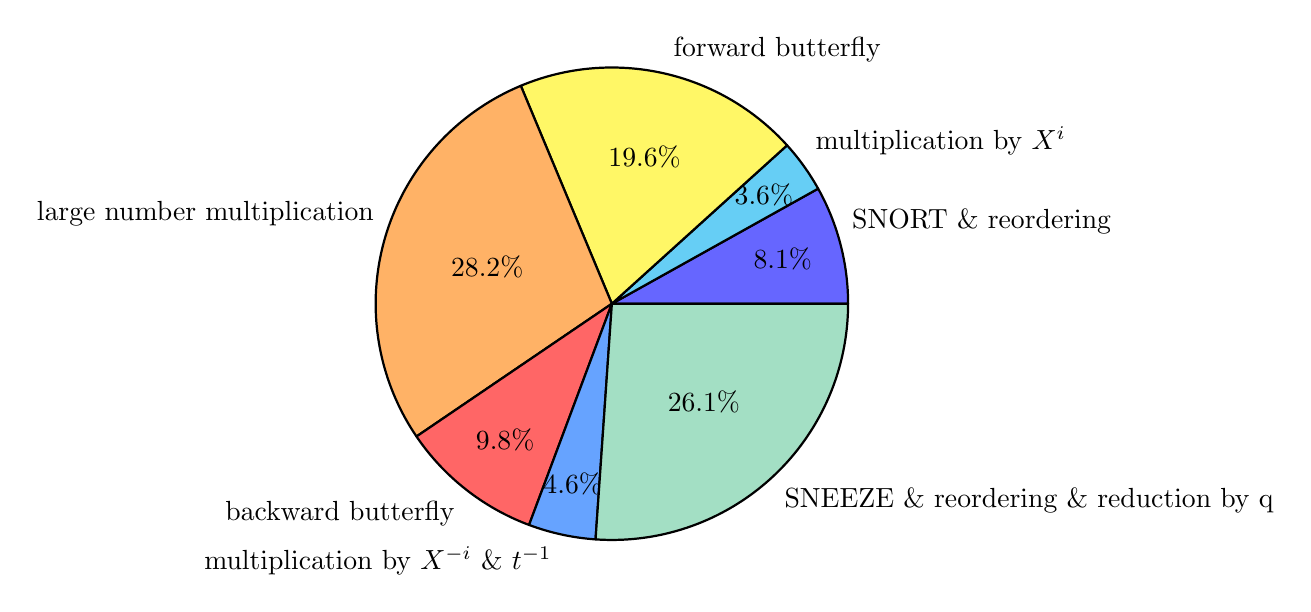
\begin{tikzpicture}

\pie[radius=3]{8.1/SNORT $\&$ reordering,
    3.6/multiplication by $X^i$,
    19.6/forward butterfly,
    28.2/large number multiplication,
    9.8/backward butterfly,
    4.6/multiplication by $X^{-i}$ $\&$ $t^{-1}$,
    26.1/SNEEZE $\&$ reordering $\&$ reduction by q}

\end{tikzpicture}

The first two steps are rather fast which is to be expected since their implementations are also relatively short and without too long loops. The forward butterfly (applied to both inputs) takes a big part of the total running time, which is also to be expected since the NTT is on of the main operations in the algorithm. It is interesting to note that the time of the forward NTT is double the time of the backward NTT (applied only to the result) which is again expected since a large part of the implementation of the two is shared and the other parts are similar. The large number multiplication is the most time consuming part, which is again expected since this is the part one tries to reduce. A larger $t$ would reduce this part even further but will increase the other steps. Step 6 turns out to be inexpensive thanks to not computing the full large number multiplication but just a multiplication by one 64-bit chunk. The last part is the surprising bit even if a couple of steps are compressed into one pass through the coefficients. To understand which parts are expensive, the following figure shows the percentage of number of cycles for each sub-step of step 7:

\vspace{5mm}

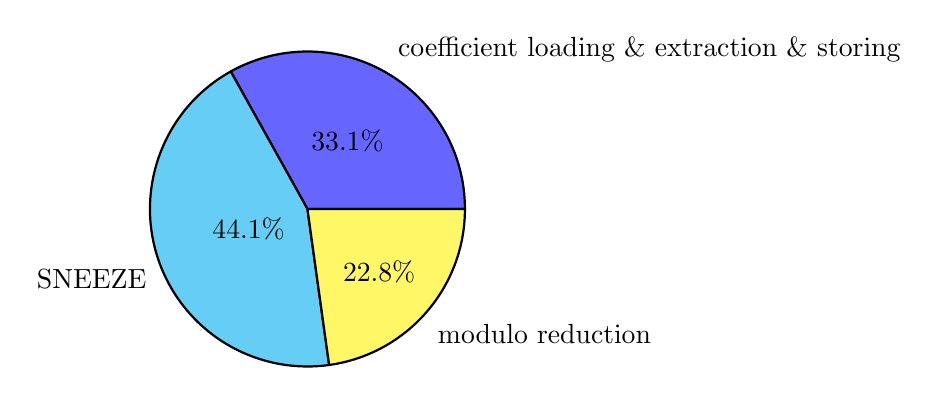
\begin{tikzpicture}

\pie[radius=2]{33.1/coefficient loading $\&$ extraction $\&$ storing,
    44.1/SNEEZE,
    22.8/modulo reduction}

\end{tikzpicture}

There are 256 numbers that need to be processed, which means running each instruction in the processing pipeline 256 times. Some instructions take 2 cycles instead of 1 as well. Reducing the code by one instruction in this setting translates into a great reduction in the number of cycles. The coefficient extraction is slow since multiple 64-bit chunks are read into WDRs instead of 32-bit registers in order to make the SNEEZE and modulo reduction simpler. The extraction alone takes 8 instructions, mostly because the instruction set is not perfectly fitted for this use case. One of these instruction takes 2 cycles, hence the extraction takes $9 \cdot 256 = 2304$ cycles. From the diagram it does not seem that one part is excessively expensive but rather all of them are moderately expensive. The issue is that there are many coefficients and the each instruction adds many cycles. Through analyzing the code in detail one may be able to reduce the number of instructions by finding another way to implement the same operations. This would make a significant improvement, but keeping in mind that the first part of the algorithm, namely preprocessing, forward NTT and the multiplication are to be executed $k$ times when the second part is executed only once (due to the aggregation in the NTT domain improvement), the issue is to some degree ameliorated.

To continue the analysis, it would be useful to imagine what would happen for other parameter choices: increasing t to 16 would decrease the numbers' widths by a factor of 2 and so the running time of the multiplication by a factor of 4. On the other hand, it would increase both the running time of steps 2, 3, 5 and 6 by a factor of 2. Computing the expected running time for the set of parameters $l=64, t=16$, it seems that the choice $t=8$ is by far better. Decreasing t to 4 would increase the running time of the multiplication by a factor of 4 but decrease the number of cycles for the other mentioned steps by a factor of 2. This makes the number of cycles of multiplication already larger than the number of cycles of the whole algorithm in the current setting. Changing $l$ to a smaller number which is not a power of 2 (since it needs to stay above 54), makes a couple of steps as the coefficient reordering, Kroneker substitution operations and others a lot more complex to implement. The extra complexity translates into more instructions which means more cycles. The difference in the numbers' widths is relatively small, hence this wouldn't be an improvement.

\section{Comparison with other implementations of polynomial multiplication schemes}

To evaluate the quality of the implementation, the overall running time is compared with a couple other implementations of polynomial multiplication schemes. One needs to keep in mind that since these other implementations are tuned for other polynomial rings, they were written with different instruction sets and have been evaluated on different hardware, the comparison is rather rough.

In the setting of Dilithium, keeping in mind that ultimately a matrix vector multiplication will be performed, the time consumption can be split into the preprocessing and forward NTT regarded together, the multiplication, and the backward NTT and postprocessing. Table \ref*{tab:comparison} shows cycle counts split into these there categories for a couple of polynomial multiplications implementations for Dilithium. It should be noted that both the Cortex M3 and M4 processors have more advanced hardware and a larger instruction set but they do not have such a large multiplier (64 bits) as OTBN has. Given that, the proposed implementation ranks pretty well in between the ones for Cortex M3 and Cortex M4.

The last entry in the table is a C implementation on OpenTitan's main processor of the polynomial multiplication as given in the Dilithium scheme. This represents the alternative to a using the big number accelerator of OpenTitan. If one holds an OpenTitan processor and wants to implement Dilithium on it, the benefit of using the implementation given in this work is clearly visible since the running time is almost three times lower and because the OpenTitan's main processor would meanwhile be free to process other things. 


\begin{table}[htpb]
    \caption[]{}\label{tab:comparison}
    \centering
    \begin{tabular}{p{0.4\linewidth} | p{0.15\linewidth} | p{0.07\linewidth} | p{0.15\linewidth} | p{0.07\linewidth}}
      \toprule
         Work & Preprocess $\&$ NTT & Mult & Postprocess $\&$ INTT & Total \\
      \midrule
         Faster Kyber and Dilithium on the Cortex-M4~\parencite{10.1007/978-3-031-09234-3_42} & 8093 & 1955 & 8415 & 18463  \\
         \hline
         \textbf{This Work} & \textbf{10763} & \textbf{9714} & \textbf{13943} & \textbf{34420} \\
         \hline
         Compact Dilithium Implementations on Cortex-M3 and Cortex-M4 ~\parencite{cryptoeprint:2020/1278} (M3 version) & 19347 & 4899 & 21006 & 45252 \\
         \hline 
         Dilithium baseline OpenTitan & 40002 & 7455 & 46649 & 94106 \\

      \bottomrule
    \end{tabular}
  \end{table}

  Aside from comparison with other implementations, it is important to note what would be the benefits of having a larger multiplier. Increasing the multiplier by a factor of two would reduce the multiplication cost by a factor of 4 which would permit to decrease t to 4 which would increase the multiplication time by a factor of 4 getting back to the current running time. The benefit would be that the number of cycles of the steps 2, 3, 5 and 6 would decrease by a factor of 2, potentially by a large amount. Increasing the multiplier to a full 256-bit size would permit to also decrease the multiplication time by a factor of 4 when keeping $t=4$. From these considerations one understands that the Kroneker+ algorithm largely benefits from having a large multiplier as RSA and ECC dedicated processors have, even if direct application of the NTT for numbers modulo $q = 2^{23} - 2^{13} + 1$ does not benefit from that.
\chapter{Conclusion}\label{chapter:conclusion}

\section{Overview}

This thesis provides an optimized implementation on the OTBN instruction set of the Kroneker+ polynomial multiplication algorithm fine tuned for the Dilithium signature scheme. It tackles various challenges from the algorithm level (choice of NTT, modulo reduction algorithm) to the implementation level (parameter choice, optimizations, lack of needed instructions). The final result is a working and efficient code that can be easily plugged into the Dilithium scheme and expected to work out-of-the-box. At the same time it provides a reference implementation of the Kroneker+ algorithm which can serve as a starting point for the adoption of other schemes on the OTBN processor. Lastly, it details on various parts of the algorithm in order to facilitate understanding from both a theoretical point of view as well as an implementation oriented perspective. 

\section{Future Work}

There are a number of improvements that can be added to this implementation in order to make it more efficient. Reduction of the number of instructions in the last step would greatly reduce the running time since they are run many times. Stopping the propagation of burrows and carries when these are 0 in some modulo reduction operations is expected to reduce the number of ran instructions by a significant amount. Combining the implementation of steps that need to load, process and save back numbers to the data memory would reduce the number of i/o interactions which are by definition slow.

One could adapt the code to other processors and instruction sets and understand which hardware capabilities are needed to make the implementation more efficient. Furthermore, the codebase used as a baseline and more implementations for other parameter sets can be developed with specific use cases, i.e. schemes in mind. 

Lastly, from a more theoretical perspective, the algorithm can be formalized and the transformations studied in more depth. One could consider maps to a ring were a other convolutions show up, as it is the case with the negative wrapped convolution. Such a study might lead to more efficient steps, or even to a completely new algorithm.
% TODO: add more chapters here

\appendix{}

\microtypesetup{protrusion=false}
% \listoffigures{}
% \listoftables{}
\microtypesetup{protrusion=true}
\printbibliography{}

\end{document}
